\input{common/preamble}

\begin{document}

% Title page, TOC, etc.
\input{frontmatter/pages}

%\chapter{Tasks}
%\section{Notes from PhD progress update}
\begin{compact_itemize}
\item MS: You have some knobs (number of depth planes, color bit-depth, LED bit-depth, Lens function, DMD framerate, decomposition algorithm, depth cues, time to render and decompose); I want to see a design space analysis, trade-offs for the various parameters in the display
\item MS: Discuss various possible approaches for scene decomposition, various possibilities choices in the optimization regime. Solve for one particular case.
\item KR: Discuss how various other display technologies can be emulated by your display
\item KR: Compare your display against other similar recent displays. Can we prove that our display is better?
\item DL,GW: Not clear what you are optimizing. Is it the depth blur? Are there other things that you could optimize for? We need to see your current optimization effort and future ones written in a much more concrete and formalized manner. 
\item LM: Discuss artifacts that may be possible in a real-time display because the different depth planes have different update rates (e.g. planes in the middle have equally spaced update rates whereas planes at the far or near have different updates - one very short and one very long)
\item GW: Need to show convergence analysis to convince folks that your algorithm actually works
\item GW: Your current approach is called projected-gradient approach
\item DL,LM: Look into error diffusion. This is a known technique in computer graphics. What you need is something like 3D error diffusion or 3D dithering.
\item LM: You can redo a lot of perceptual experiment with this display. You're holding yourself back by not doing them. Such studies would be real contribution to science rather than engineering which is what most of your work is about.
\item TW, MS: Please share with us a block diagram of your real-time system
\end{compact_itemize}

\section{Tasks}
\begin{compact_todolist}
\item Write down these algorithms for color-adaptive decomposition:
\begin{compact_todolist}
\item Mixed-primary heuristic approach
\item Highest energy channel heuristic approach
\item Mixed-primary projected gradient approach
\item Highest energy channel projected gradient approach
\end{compact_todolist}
\item Also write down the fixed-pipeline algorithm
\item Include pictures to compare the four algorithms
\item Write code to calculate focal stacks
\item Make blockdiagram of the real-time system. Share it with the PhD committee
\end{compact_todolist}

\chapter{Introduction}
\label{chapter:introduction}
Augmented Reality (AR) systems offer unprecedented experiences and promise to augment the physical world around us with digital content seamlessly. Providing a seamless, perceptually realistic experience, however, requires the display to support all depth cues of the human visual system~\cite{Palmer:1999,Howard:2002} accurately. While current AR displays offer impressive capabilities, they typically do not support important depth cues such as accommodation or occlusion.

Accommodation is the depth cue that results from the ability of the lens in the eye to focus to different depths of the real world. For improved realism, an AR display should be capable of optically presenting a 3D virtual scene such that the user could explore the virtual scene by focusing to different depths.

Occlusion is the depth cue that arises from solid objects blocking rays of light that arise from real-world points behind it. Providing accurate, i.e., mutually consistent and hard-edge, occlusion between digital and physical objects with optical see-through AR displays is a significant challenge. When digital content is located in front of physical objects, the former usually appear semi-transparent and unrealistic (see Fig.~\ref{fig:varifocal_occlusion:results}, columns~1 and~2). To adequately render these objects, the light reflected off of the physical object toward the user has to be blocked by the display before impinging on their retina. This occlusion mechanism needs to be programmable to support dynamic scenes, and it needs to be perceptually realistic to be effective. The latter implies that occlusion layers are correctly rendered at the distances of the physical objects (see Fig.~\ref{fig:varifocal_occlusion:depth-dependent-occlusion}), allowing for pixel-precise, or hard-edge, control of the transmitted light rays.

Display technologies that provide these depth cues could revolutionize the way we communicate, visualize and interact with digital information, e.g., \emph{telepresence} systems will significantly benefit from being able to depict occlusion~\cite{maimone2013general}, \emph{visualization} of 3D data, especially data composed of surfaces within surfaces such as that of the human anatomy would greatly benefit from occlusion as well as accommodation depth cues.

\section{Contributions}
The broad contributions of this dissertation are new optical designs, new real-time rendering algorithms, and prototype displays that demonstrate accommodation and mutual occlusion depth cues over an extended depth-range.

For accommodation, this dissertation's contributions are: (1) A volumetric NED exhibiting 280 perceptually simultaneous binary depth planes, each an arbitrary RGB color, situated between 15~cm (6.7 diopters) and 400~cm (0.25 diopters) from the viewer. (2) A rendering pipeline that decomposes a 3-D scene into the set of single-color binary depth planes, such that 24 bpp color voxels are displayed at 280 unique depth positions. (3) A yet-to-be-developed color-adaptive decomposition algorithm for the NED which also demonstrates intra-pupillary occlusions.

For depth-dependent occlusion, this dissertation's contributions are: (1) Varifocal occlusion as an AR display capability that adaptively changes the focal distance of an occlusion mask to enable depth-dependent hard-edge occlusion. (2) Complementary approaches of optimization and closed-form solutions for arriving at an optical design that enables a focus-tunable optical system to achieve varifocal occlusion in a perceptually realistic manner without optically distorting the observed scene. (3) A monocular varifocal occlusion-capable AR display prototype that demonstrates improved realism through depth-dependent occlusion over a large depth range (30~cm to 300~cm).


\section{Thesis Statement}
The use of computational displays, where the optics, electronics, and algorithms are co-designed, will improve accommodation and occlusion in AR displays. 


\chapter{Background}
\label{chapter:background}
Coming soon \dots

\begin{comment}
\section{Literature on the importance of depth cues for AR displays}

\cite{sielhorst2008advanced} provide a good set of references on depth perception studies. \cite{sielhorst2008advanced} also provide a good summary of \cite{cutting1995perceiving} which in turn is a seminal paper about the different types of depth cues and their relative importance. The summary: Occlusion is the most important depth cue even though it is only an  because because it can only reveal the order but not a relative or absolute distance. \cite{sielhorst2008advanced} call it ``interposition''. \cite{sielhorst2008advanced}.
\end{comment}


\chapter[Volumetric Augmented Reality Display]{Volumetric Augmented Reality Display\footnote{Most of this chapter previously appeared as an article in Transactions on Visualization and Computer Graphics. The new sections of this chapter are adaptive color-to-binary decomposition (Sec.~\ref{sec:volumetric:acd}) and a real-time display (Sec.~\ref{sec:volumetric:rts}). The original citation is as follows: \bibentry{Rathinavel2018}}}
\label{chapter:volumetric_ned}
\section{Introduction}
\label{sec:volumetric:introduction}
Near-eye displays that seamlessly integrate virtual content into the real world offer exciting possibilities. Real-virtual integration could induce a paradigm shift in multiple aspects of our lives, including education, communication, entertainment, and others. Near-eye displays, as compared to spatially augmented reality and 3-D displays, allow true immersion in the sense that the near-eye display user could truly experience a virtual world around them in all directions while preserving the user's natural experience and view of the real world. However, several challenges must be addressed to realize truly immersive see-through near-eye displays. One of these is the mismatch between the vergence and accommodation cues of depth perception. Vergence is the orienting of our eyes such as to center the image of a fixated object on the fovea. Accommodation is the eye lenses' ability to change their focal length to bring the object of fixation into proper focus on the retina. These are cross-coupled physiological effects. Their absence, mismatch, or incorrect representation (may also apply to other depth cues) can disrupt the sense of presence or immersion and may cause visual discomfort, eyestrain, and nausea~\cite{Hoffman2008Vergence}. 

Some of the proposed solutions to the problem of providing such depth cues attempt to approximate focus cues. Varifocal displays, monovision displays, and even some implementations of multifocal displays are in this category. Some other proposed solutions, such as light field displays and holographic displays, provide accurate focus cues but have limitations. Current implementations of light field displays have poor resolution or are diffraction-limited. Current implementations of holographic displays are compute-intensive and may have very small eyeboxes. Phase-only spatial light modulator (SLM) technologies also need improvement before holographic displays based on these technologies can become practical.

This paper explores a new class of displays: volumetric near-eye displays. Our approach is to sweep the virtual image plane back and forth over a wide range of diopters and use high-speed DMDs coupled with high-speed illumination to present a large number of multiple thin slices of a computer generated volume. While this sounds similar to multifocal displays that show images at various fixed depths, there is a crucial difference:

Traditionally, for multifocal displays, the computer-generated volume is decomposed into a series of image planes placed at different depths; for time-multiplexed multifocal displays, this necessitates that the focus-tunable lens or deformable mirror settle down in each focus state. Our approach is to oscillate the focus-tunable lens in a continuous state and display a stack of binary images at high-speed such that the displayed stack of images is perceived as slices of a continuous full-color volume. We decompose the computer-generated volume locally, on a per-voxel basis, and distribute the decomposition around the location of the voxel. Thus, our rendering algorithm is aware of and leverages the fact that the focus-tunable lens is in continuous motion--rather than assuming a lens that moves and settles in discrete steps. Low-level hardware access to a high-speed DMD and a high-speed HDR RGB LED light source allows control of display pattern and illumination for each binary frame. We present a rendering pipeline for volumetric near-eye displays that utilize such hardware.

One might be concerned about the computational complexity of our approach. In our implementation, we make some simplifying assumptions to reduce computational overhead. However, these simplifications might not be desirable in a human-wearable product; without these assumptions, our approach would be moderately computationally demanding. While this might be an encumbrance for today's embedded hardware, we assert that near-eye displays (NEDs) of the future must have substantially more compute power to perform, e.g., low-latency corrections, head and eye tracking, real-world scene understanding, and so on. For example, onboard GPUs are already found in NEDs such as Microsoft HoloLens. While our current implementation is offline, we believe that future NEDs will have sufficient onboard computational resources to perform the required computations in real-time on the device.  
% * <blate@cs.unc.edu> 2018-06-19T15:37:20.027Z:
% 
% > moderately computationally demanding
% 
% Quantify, at least relative to the simplified approach... e.g., without these simplifications, computational requirements increase on the order of X percent. 
% 
% ^.

\subsection{Contributions}
\label{sec:Contributions}
This paper's main contributions are: 

\begin{enumerate}
\item A volumetric NED exhibiting 280 perceptually simultaneous binary depth planes, each an arbitrary RGB color, situated between 15cm (6.7 diopters) and 4M (0.25 diopters) from the viewer.
\item A rendering pipeline for the new NED that decomposes 3-D graphics primitives efficiently into the set of single-color binary depth planes, such that 24 bits-per-pixel color voxels can be displayed at 280 unique depth positions.
\end{enumerate}

\begin{comment}
\begin{enumerate}
\item We describe a new rendering pipeline for binary multifocal displays that allows a color voxel to be decomposed into a dense set of binary voxels in a small region around the color voxel. 
We reject the traditional notion that the color volume should be decomposed into a sparse set of color image planes, each located at a different depth. 
We analyze the losses in depth and spatial resolution that might result from the proposed decomposition and discuss mitigation methods.
\item We introduce volumetric NEDs capable of presenting high-resolution color imagery in a \emph{perceptually continuous} depth range across a large range of diopters. We demonstrate a prototype system that displays a 24-bits-per-pixel image in a binary volume composed of 280 focal planes distributed over a depth range of 15cm (6.7 diopters) to 4M (0.26.7 diopters), refreshed at 60 Hz. 
\end{enumerate}
\end{comment}

\subsection{Benefits}
\label{sec:benefits}
In addition to supporting the current volumetric display implementation, our proposed system can emulate varifocal displays and previous multifocal displays. This could allow the system to become a test-bed for future perceptual studies on accommodation. Our display allows low-level access to many stages of the graphics pipeline between GPU and the actual emission of light rays that form a retinal image. This low-level access could be used to study alternative rendering pipelines for future near-eye displays and advanced projectors. Integration of our present work and previous work with similar hardware~\cite{Lincoln2016motion,Lincoln2017scene} could lead to a near-eye display with several desirable properties (low-latency, high dynamic range, accommodation-capable). 



\section{Related Work}
\label{sec:volumetric:related_work}

\subsection{Volumetric Displays}
\label{sec:volumetric:volumetric_displays}

Volumetric displays create multiple real or virtual light sources in a three-dimensional volume of space and can typically be seen from a wide range of angles around the display. These light sources are the 3-D analog of pixels and are called \emph{voxels}. Earlier designs of volumetric displays were table-top designs and the displayed volume was confined to the \emph{physical volume of the display}~\cite{Favalora2002100, Sullivan2004Depthcube, Cossairt2007Geometric, Ochiai2016Fairy, Refai2009Static, Smalley2018photophoretic}. One of the limitations of most of these displays is that the light sources are presented additively and view-dependent effects, such as occlusion, are absent. This limitation is overcome in Cossairt et al.~\cite{Cossairt2007Geometric} and in Jones et al.~\cite{Jones2007Rendering} by using anisotropic diffusers.

Our proposed display provides a methodology to create virtual light sources over an \emph{extended volume external} to the display's physical volume. Applied to near-eye displays, this methodology has the potential to solve the vergence-accommodation conflict and reduces the need to track accommodation state in future eye-tracking technology. To clarify, our display needs eye-tracking in the sense that the \emph{pupil position} must be tracked, but the \emph{accommodation state} of the pupils need not be tracked.

\subsection{Accommodation supporting NEDs}
\label{sec:volumetric:accommodation_neds}
\subsubsection{Multifocal near-eye displays}
\label{sec:volumetric:multifocal_displays}

Multifocal near-eye displays, first proposed by Akeley et al.~\cite{Akeley2004stereo}, display a small number of images at different depths; the images are perceived additively~\cite{Akeley2004stereo,MacKenzie2010Accommodation,Liu2010novel,Love2009high,Hu2015Design}. In Akeley, et al.~\cite{Akeley2004stereo} and MacKenzie, et al.~\cite{MacKenzie2010Accommodation}, subregions of an LCD panel were mapped to different focal planes using beamsplitters. Liu and Hua~\cite{liu2009time}, Love et al.~\cite{Love2009high}, and Liu et al.~\cite{Liu2010novel} propose a switchable lens to multiplex between the multiple focal planes. Wang et al.~\cite{wang2018digitally} propose a segmented lens and a fast optical shutter to create the focal planes.  Hu and Hua~\cite{Hu2014design,Hu2014High,Hu2015Design} propose to use high-speed optical components, such as a DMD and a 1KHz deformable membrane mirror, to achieve a larger number of focal planes (six) than previously demonstrated. 

Because a relatively small number of depth planes are used to represent objects occupying a large volume, multifocal plane displays need scene decomposition algorithms to optimally represent a 3-D scene using a few 2-D image planes. Content generated by these scene decomposition algorithms provide synthetic focus cues to represent objects that lie in between the focal planes. MacKenzie et al.~\cite{MacKenzie2010Accommodation} propose a per-pixel linear blending approach. Narain et al.~\cite{Narain2015optimal} propose an optimized blending algorithm that can demonstrate occlusion, reflection, and non-Lambertian effects. Mercier et al.~\cite{Mercier2017Fast} and Lee et al.~\cite{Lee2017foveated} propose a new scene decomposition techniques that are tolerant to eye movements. While scene decomposition algorithms help to depict imagery that lie between the focal planes, the spatial frequency of the fused image is inversely related to the focal plane separation~\cite{Hu2014design, Hua2017Enabling}. 

Similar to multifocal displays, our display can also be thought of as a view-dependent and depth-fused multifocal display. Our display has about two orders of magnitude more focal planes than previous multifocal displays which approaches a \emph{volumetric display's} performance. Like previous multifocal displays, our display also requires eye-tracking to provide correct occlusion and dis-occlusion effects. In this paper, we assume that the pupil position is known. Like previous multifocal displays, we also share the problem of generating synthetic focus cues through scene decomposition to represent a large 3-D scene with 2-D image planes. However, while previous methods perform the scene decomposition in an image-oriented manner, we perform the scene decomposition in a voxel-oriented manner. This is discussed in detail in Section~\ref{sec:volumetric:rendering_pipeline}. 

Matsuda et al.~\cite{Matsuda2017focal} propose a multifocal display whose focal surfaces can acquire non-planar, scene-dependent surface geometry. Matsuda et al.~\cite{Matsuda2017focal} propose a rendering pipeline that converts a 3-D scene to multiple piecewise smooth 2-D surface representations that are displayed in a time-multiplex manner. In comparison with their work, our rendering pipeline generates a single 2-D surface representation of the 3-D scene, and our display does not require piecewise smooth 2-D surfaces. Our display also exhibits more uniform image quality throughout the displayed volume. 

Recently, Lee et al.~\cite{Lee2018Tomoreal,Lee2018Shape} propose a multifocal plane display which uses synchronized DMD, LCD panel, and focus-tunable lens. With the exception of their LCD panel and our HDR LEDs, the hardware and operation seem similar to our display. But, because of their use of LCD panel and our use of HDR LEDs, the rendering pipelines of the two displays are different. In their display, during the focus-tunable lens' cycle, the DMD panel is used to illuminate portions of the LCD panel resulting in color sub-images at various depths. In our display, during the focus-tunable lens' cycle, the HDR LEDs and DMD create a series of single-color binary images which integrate together such that a color volume is perceived. 


\subsubsection{Light field near-eye displays}
\label{sec:volumetric:light_field_displays}
Light field displays synthesize the individual light rays that recreate the 3-D scene and can conceptually provide accurate focus cues and monocular occlusion. However, current implementations of light field displays are diffraction-limited~\cite{Maimone2014Pinlight,Huang2015Light} or have poor resolution due to a spatial-angular resolution trade-off~\cite{Lanman2013near,Hua2014Three}. While light field displays present a virtual pixel by displaying the light rays originating from the virtual pixel individually, our volumetric NED displays the entire set of light rays that originate from the virtual pixel simultaneously.

\subsubsection{Holographic near-eye displays}
\label{sec:volumetric:holographic_displays}

Holographic displays precisely modulate the wave function of the image arriving at the pupil using a digital hologram displayed on a phase-only spatial light modulator (SLM) such as a phase-only liquid crystal on silicon (LCoS) panel. Conceptually, these displays can also provide accurate focus cues, monocular occlusion, vision correction, and non-Lambertian effects. Current implementations of holographic near-eye displays have a very small eyebox~\cite{Maimone2017Holographic}, and are computationally expensive~\cite{Shi2017Near,Maimone2017Holographic,Matsuda2017focal}. Our NED also has a small eyebox (4mm) and is moderately computationally intensive. Our NED's eyebox can be larger; the limiting factor for our eyebox is the focus-tunable lens's aperture (1cm). Maimone et al.~\cite{Maimone2017Holographic} demonstrate a NED that can provide per-pixel focus cues for a range of 10cm to 32.5cm. In comparison, our NED provides per-pixel near-accurate focus cues for a large depth range (15cm to 4M).

\subsubsection{Varifocal near-eye displays}
\label{sec:volumetric:varifocal_displays}
Varifocal near-eye displays have a single image plane where the vergence and focus cues match, and this plane is moved by using focus-tunable lenses~\cite{Padmanaban2016Optimizing,Liu2008Optical,Konrad2016Novel}, or deformable membrane mirrors~\cite{Dunn2017Wide}, or by actuating fixed-focus optical components~\cite{Aksit2017Near}. In a varifocal display, all pixels are at the same focal plane - so virtual pixels that do not lie on the plane of focus need to be synthetically blurred in proportion to their distance from the plane of focus. Varifocal displays need to track the accommodation state of the pupil~\cite{Padmanaban2016Optimizing} or assume that the pupils are accommodated to the eye convergence distance~\cite{Dunn2017Wide,Aksit2017Near}. 

\subsection{Rendering pipeline for DMD-based NEDs}
Previous NEDs have used DMDs and proposed different rendering pipelines~\cite{Lincoln2016motion,Lincoln2017scene,Hu2014design,Hu2015Design}. We build upon their hardware but propose a new rendering pipeline. A detailed discussion is provided in Section~\ref{sec:volumetric:previous_rendering_pipeline}.


\section{System Overview}
\label{sec:volumetric:system_overview}
Figure~\ref{fig:volumetric:proposedCandidate} shows an overview of our NED's hardware and operation. Our proposed display consists of three main active optical components namely: (1) an HDR Illuminator, (2) a DMD chip, and (3) a focus-tunable lens. These three optical components are driven at high-speed by an FPGA, a microcontroller, and custom electronics. 

The focus-tunable lens is driven in a continuous mode such that its optical power follows a triangular or sinusoidal waveform. The DMD projector is synchronized with the focus-tunable lens to display a stack of binary frames in each lens cycle, and the HDR illuminator illuminates the DMD chip with a distinct selected RGB color for each binary frame. Each cycle of the focus-tunable lens is one frame of the overall display. To avoid confusion, each frame of the DMD will be referred to as \emph{single-color binary image} whereas the 24-bit color rendering of the 3-D scene will be referred to as the color image.

Our DMD's refresh rate is $f_{\text{DMD}} = 16,800$ Hz, and our target display refresh rate is $f_{\text{NED}}=60$ Hz. Then the number of single-color binary images displayed by the DMD in each frametime of the NED is given by
\begin{equation}
N_b = \frac{f_{\text{DMD}}}{f_{\text{NED}}} = 280.
\label{eq:280}
\end{equation}

These $280$ single-color binary images are distributed in depth along the user's line-of-sight from 15cm to 4M.  Correct modeling of the depth distribution and field-of-view (FoV) of binary images is necessary for proper rendering and color decomposition. 

The optical design of our NED is discussed in Section~\ref{sec:volumetric:Optical_design} and the rendering pipeline that converts 3-D scene information into multiple single-color binary images is discussed in Section~\ref{sec:volumetric:rendering_pipeline}. 


\section{Optical Design}
\label{sec:volumetric:Optical_design}
This section models the optical design and timing characteristics of our near-eye volumetric display to arrive at the geometry of the displayed volume, i.e., depth distribution and FoV of the binary images. The geometry of the volume is used in the rendering pipeline to decompose a 3-D scene to a volume that is displayed by the NED.

\begin{figure}
\centering
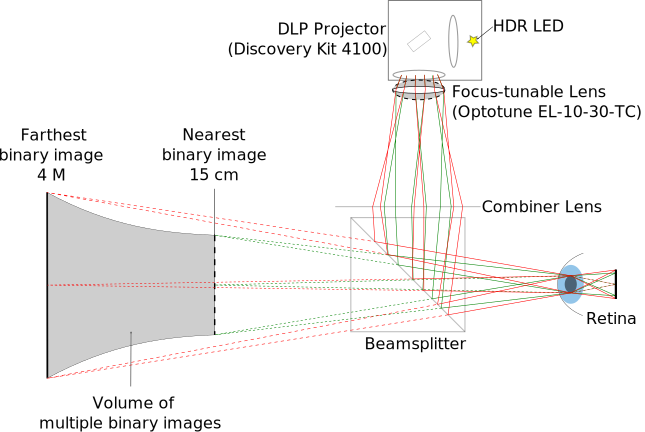
\includegraphics[width=0.99\columnwidth]{images/volumetric/proposedCandidate}
%\fbox{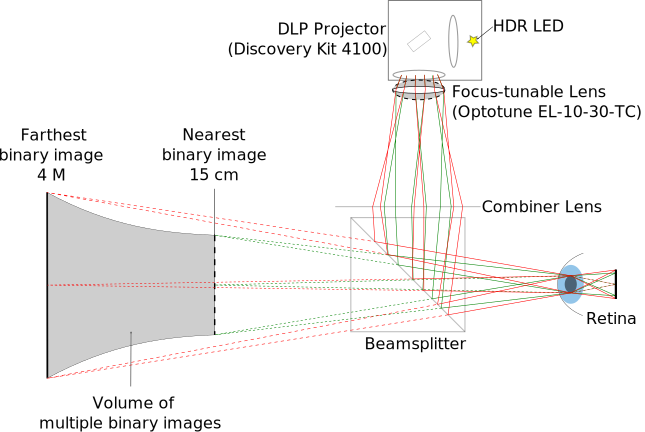
\includegraphics[width=0.46\textwidth]{images/volumetric/proposedCandidate}}
\caption[Volumetric NED: optics overview]{Figure shows an overview of the hardware and operation of our NED. The NED is composed of a high-speed HDR LED, high-speed projector, focus-tunable lens, and other common optical components. The NED's optics, rendering pipeline, and the synchronized operation of its active components (HDR LEDs, DMD, focus-tunable lens) work together to present a color volume spanning 15cm (6.7 diopters) to 4M (0.25 diopters).}
\label{fig:volumetric:proposedCandidate}
\end{figure}

\subsection{Overview of optical design} 
Our optical system is composed of multiple lenses (see Figure~\ref{fig:volumetric:unfolded}). The left diagram of Figure~\ref{fig:volumetric:unfolded} shows the image formation process for any projector. Such a projector can be converted to a near-eye display by placing an eyepiece or combiner lens just after the projected image. Since the projected image for most off-the-shelf projectors would be too large, a converging lens could be placed between the projector and the combiner lens; this helps in reducing the magnification of the projected image and in reducing the form-factor of the NED. In our NED, instead of placing a static converging lens between the projector and the combiner lens, we place a focus-tunable lens (see right diagram of Figure~\ref{fig:volumetric:unfolded}) and configure the optical power of the focus-tunable lens to sweep the real image of the DMD close to the combiner lens. To see a virtual image, the combiner lens's focal length has to be less than the distance between the lens and the real image (i.e., $f_3 < o_3(t)$).

\subsection{Modeling of optical design to derive volume geometry}
We begin with stating the Gaussian thin-lens equation
\begin{equation}
\frac{1}{f} = \frac{1}{o} + \frac{1}{i},
\label{eq:basic_optics_equation}
\end{equation}
and associated equations
\begin{equation}
i = \frac{f o}{o - f},\quad M = \frac{I}{O} = -\frac{i}{o},
\label{eq:basic_optics_equation_2}
\end{equation}
where $f$ denotes focal lens of a thin lens, $o$ denotes object distance, $i$ denotes image distance, $O$ denotes the object size, $I$ denotes image size, and $M$ denotes the magnification of the lens.

\begin{figure*}
\centering
%  \fbox{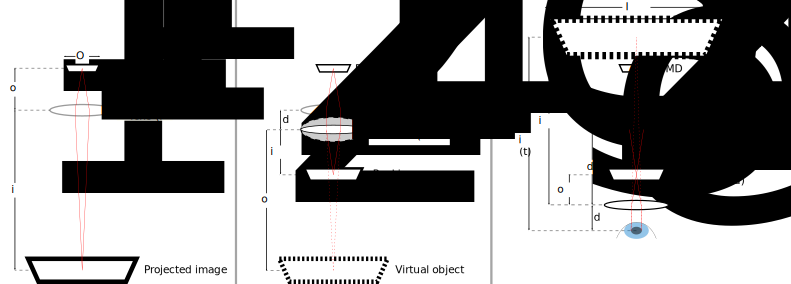
\includegraphics[width=0.46\textwidth]{images/volumetric/unfolded}}
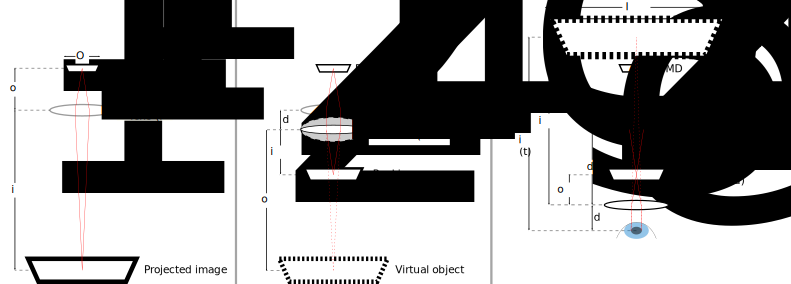
\includegraphics[width=0.95\textwidth]{images/volumetric/unfolded}
\caption[Volumetric NED: unfolded optics]{Our NED's optics can be analyzed in three stages. Figure shows the unfolded optics and ray diagram for each stage. \emph{Left: } Image formation for the DMD projector using manufacture-provided projection optics. \emph{Middle: } Adding a focus-tunable lens at the exit pupil of the DMD projector causes the real image of the DMD to be formed closer; Configuring the focus-tunable lens power to continuously oscillate causes the real image of the DMD to also oscillate. \emph{Right: } A combiner lens finally creates a virtual image of the DMD that can be seen by the eye.}
\label{fig:volumetric:unfolded}
\end{figure*}


\begin{figure}[tb!]
\centering
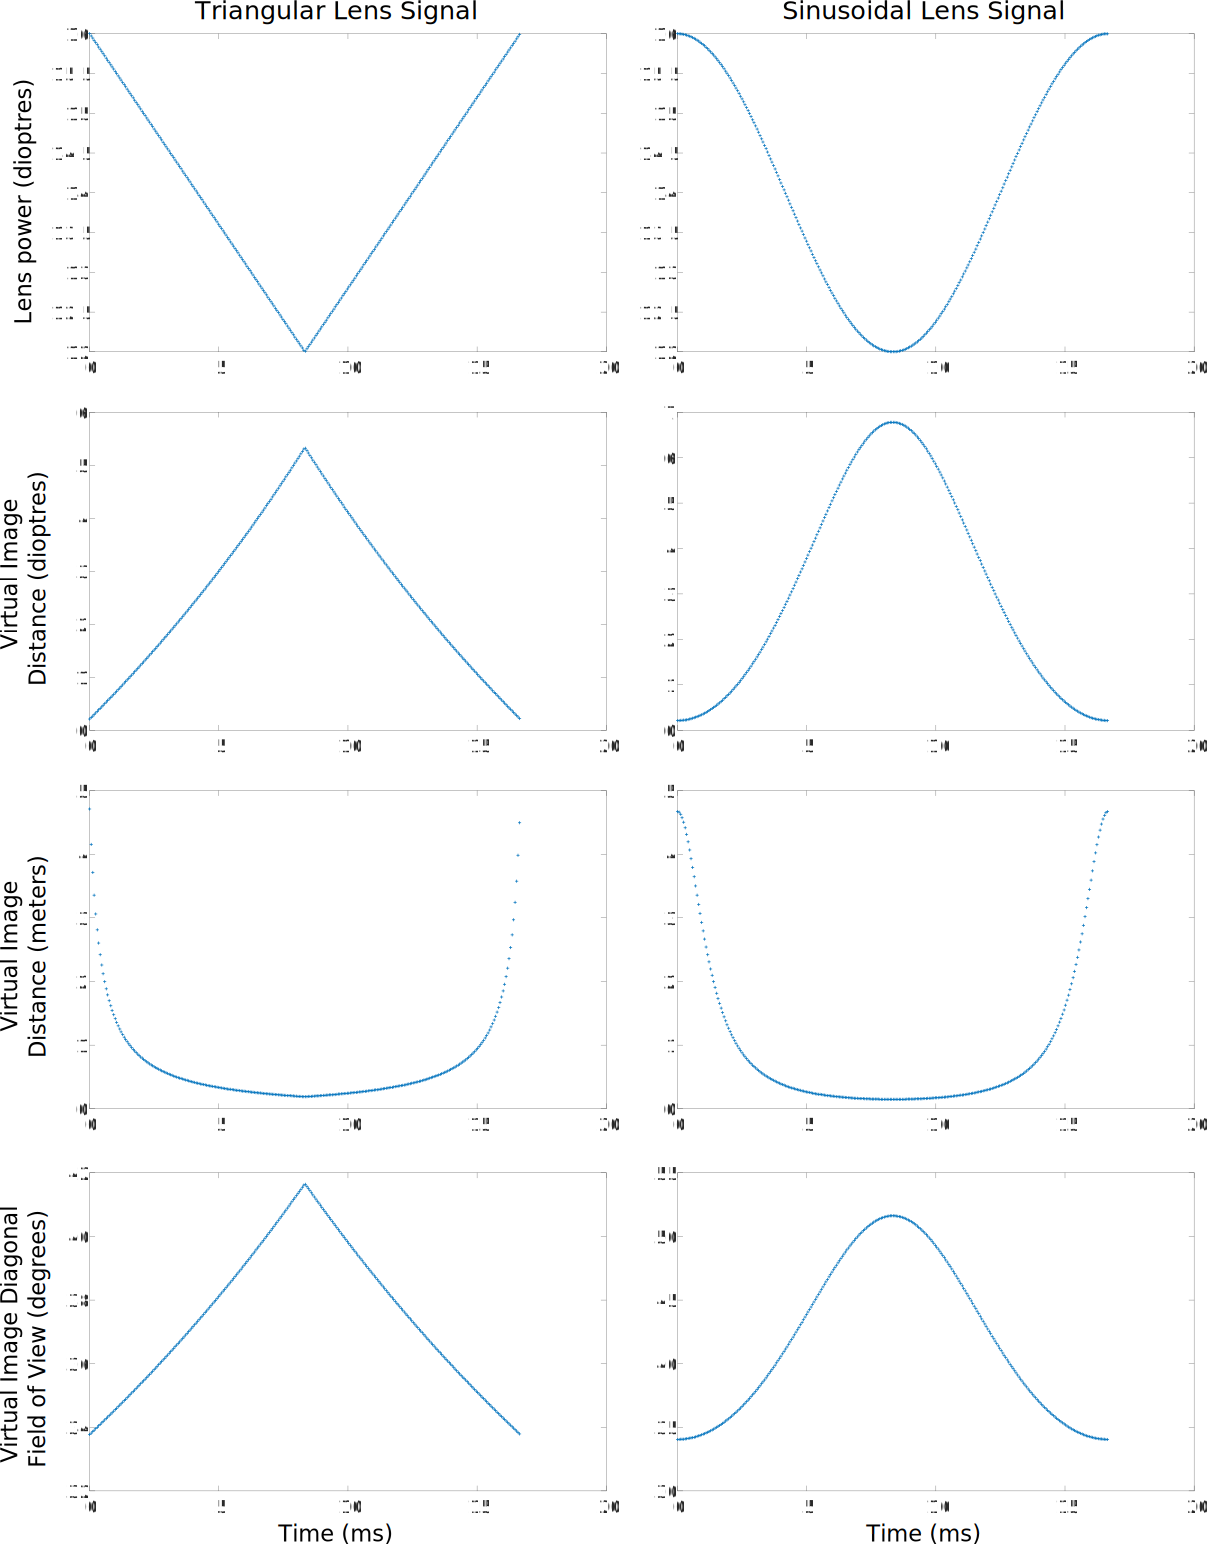
\includegraphics[width=0.9\textwidth]{images/volumetric/graphs}
\caption[Volumetric NED: graphs modelling display's depth plane distribution and FoV]{Graphs modeling the depth distribution and FoV of the displayed single-color binary images that compose the volume formed by synchronizing the DMD projector and a continuously oscillating focus-tunable lens. The oscillating lens's optical power can follow a triangular waveform \emph{(Left column)} or a sinusoidal waveform \emph{(Right column)}. Data presented in these graphs are used in the rendering pipeline to convert 3-D scene information to multiple single-color binary images that are displayed by the NED. Equations used to generate these graphs are described in Section~\ref{sec:volumetric:Optical_design}.}
\label{fig:volumetric:graphs}
\end{figure}




Due to the presence of multiple lenses in the optical stack (see Figure~\ref{fig:volumetric:unfolded}), we analyze the image formation of each lens separately and consider the image formed by each lens as the object for the next lens. This gives the following geometric relations:
\begin{equation}
o_2 = i_1-d_1, \quad o_3(t) = d_2 - i_2(t), \quad i_e(t) = i_3(t) + d_e.
\label{eq:geometric_relations}
\end{equation}

The relationship between the distance from the DMD to the projection lens ($o_1$), focal length of the projection lens $f_1$, and the projected image distance ($i_1$) is given by
\begin{equation}
i_1 = \frac{f_1 o_1}{o_1 - f_1}.
\label{eq:img1}
\end{equation}

The relationship between the object distance $o_2 = i_1 - d_1$, focal length ($f_2(t)$), and image distance ($i_2(t)$) for the focus-tunable lens is given by
\begin{equation}
i_2(t) = \frac{f_2(t) o_2}{o_2 - f_2(t)} = \frac{f_2(t) (i_1 - d_1)}{(i_1 - d_1) - f_2(t)}.
\label{eq:img2}
\end{equation}

The optical power of the focus-tunable lens ($f_2(t)$) can be configured to maintain a constant value or follow a time-varying square, triangular, or sinusoidal waveform. Other waveforms may be possible with custom electronics, but for this chapter, we analyze only the triangular and sinusoidal waveforms of lens power.

To define optical power of the focus-tunable lens as a function of time, we define some standard parameters for time-varying signals: \emph{DC bias}, \emph{amplitude}, and \emph{half-time period}. Let the DC bias, which is the average value of the signal over one full-time period be denoted by $D$. Let the amplitude, which is half of the peak-to-peak value, be denoted by $A$. Note that each cycle of the lens is the frametime of the NED. Hence, the frequency of the lens is equal to the refresh rate of the NED ($f_{\text{NED}}$). Let $a$ denote half a time period ($a = \frac{1}{2f_{\text{NED}}}$). The optical power of the focus-tunable lens, when following a triangular waveform, can be modeled as
\begin{equation}
f_2(t) = D - A\left(\frac{1}{2} - \left|\frac{t - a}{a}\right|\right),
\label{eq:general_triangular}
\end{equation}

and when following a sinusoidal waveform, it can be modeled as
\begin{equation}
f_2(t) = D + A\text{sin}(2\pi f_{\text{NED}} t).
\label{eq:general_sinusoidal}
\end{equation}

And finally, the relationship between the object distance ($o_3(t)$), focal length ($f_3$), and image distance ($i_3(t)$) for the combiner lens is given by
\begin{equation}
i_3(t) = \frac{f_3 o_3(t)}{o_3(t) - f_3} = \frac{f_3(i_2(t) + d_2)}{(i_2(t) + d_2) - f_3}.
\label{eq:img3}
\end{equation}

The above equations~\eqref{eq:geometric_relations} to \eqref{eq:img3} are sufficient to calculate the depth of each binary image plane. The FoV of the virtual binary images is found by repeated application of the magnification formula from  Equation~\eqref{eq:basic_optics_equation}:
\begin{equation}
M = M_1M_2M_3,
\label{eq:combined_magnification}
\end{equation}

\begin{equation}
I_e = MO_1,
\label{eq:virtual_image_size}
\end{equation}

\begin{equation}
\theta_{\text{FoV}} = 2\text{tan}^{-1}\left(\frac{I_e}{2i_e}\right).
\label{eq:fov}
\end{equation}

In our system, these are the values for the known quantities: $f_{\text{DMD}} = 16,800$ Hz, $f_{\text{NED}} = 60$ Hz, $f_1 = 2.96$cm, $o_1 = 3$cm, $O_1 = 1.778$cm (diagonal size of the DMD module), $d_1 = 3$cm, $f_3 = 6$cm, $d_2 = 12$cm, $d_e = 3$cm, $D = 14$, $A = 4$, and $a = 8.33$ ms. Equations~\eqref{eq:280} to \eqref{eq:fov} are evaluated with the above values to calculate the geometry of the displayed volume. The geometry of the volume is graphed in Figure~\ref{fig:volumetric:graphs}. 

The above formulation and graphs in Figure~\ref{fig:volumetric:graphs} shows only 140 unique depth planes over the time period because depth values in the first half of the time period are repeated in the second half of the time period. Our implementation is slightly different from this - we apply a small phase difference to equations~\eqref{eq:general_triangular} to \eqref{eq:general_sinusoidal} to get 280 unique depth values. 

\subsection{Sinusoidal vs. triangular waveforms}
\label{sec:volumetric:sinusoidal_vs_triangular}
In optical imaging systems, including the human eye, the blur of an object that is defocused is directly proportional to the difference between the actual distance of focus and the distance of the object in units of diopter. In our NED, the depth distribution of images should ideally be dioptrically equidistant from each other. From Figure~\ref{fig:volumetric:graphs}, it can be seen that the lens power following a triangular waveform results in a near-linear and equidistant distribution of virtual image planes in dioptric space. Hence, we implemented the rendering pipeline and electronic synchronization assuming that the lens sweeps a triangular waveform. However, when we used the sinusoidal waveform in place of a triangular waveform, keeping everything else such as the color decomposition, and electronic synchronization the same, we didn't notice a significant difference in the displayed volume geometry and image quality. This may be either because the difference between the triangular and sinusoidal waveforms is negligible compared to the minimum dioptric difference required to make a perceptual difference or because the lens' triangular and sinusoidal waveforms are similar, which can often happen with physical systems due to inertia/friction, etc., especially at higher frequencies.

\section{Rendering Pipeline}
\label{sec:volumetric:rendering_pipeline}
In this section, we first discuss the rendering pipelines of previous DMD-based NEDs, then describe our full rendering pipeline from graphics primitives to single-color binary images, and finally discuss the benefits and limitations of our rendering pipeline.

\subsection{Rendering pipeline for previous DMD-based NEDs}
\label{sec:volumetric:previous_rendering_pipeline}


% Main constraint in binary multifocal displays
% Previous rendering pipelines
\subsubsection{Low latency and HDR NEDs}
Most display technologies that employ a DMD also use a constant intensity or bivalent illumination source and use pulse train modulation to create grayscale or color imagery~\cite{Lincoln2016motion}. Recently, Lincoln et al.\cite{Lincoln2017scene} demonstrated a DMD-based display system which used a controllable high-speed HDR illuminator. They demonstrated that the intensity and color of the illumination could be changed over a wide range on a per-binary frame basis. They also proposed a new color to binary decomposition method, which they call \emph{Direct Digital Synthesis (DDS)}. Let $d$ be the desired color intensity value, $g$ be the generated color intensity value, and $s$ be the step index of the binary representation of the value of $d$. Then, DDS decomposition from color to binary values can be represented per color channel as shown below: 

\begin{equation}
g = \sum_{s = 0}^{n-1} \left(2^s \times \text{bit}(d,s)\right).
\end{equation}

\subsubsection{Multifocal plane NEDs}
Previous DMD-based multi-focal plane displays~\cite{Hu2014design,Hu2015Design} decomposed a 3-D scene to a stack of \emph{color images} fixed at the various depths. In these approaches, the focus-tunable lens or deformable membrane mirrors would step through a set of focal lengths, and at each focal length, \emph{after the lens stabilizes}, a series of binary images was displayed by one of the classical pulse train modulation schemes to generate color imagery. For such color image plane based approaches, we provide equations below for the relationship between the DMD's framerate ($f_{\text{DMD}}$), number of focal planes ($N_{\text{planes}}$), framerate of the NED ($f_{\text{NED}}$), and the color depth per color channel ($N_{\text{gray}}$). Up to some extent, a multifocal NED with a larger number of $N_{\text{planes}}$ can present better imagery because the scene decomposition algorithms of depth fused multifocal displays trade-off the spatial frequency of the fused image and the focal plane separation~\cite{Hu2014design,Hua2017Enabling}. 

In case of classical pulse train modulation schemes, the number of focal planes is given by
\begin{equation}
N_{\text{planes}} = \frac{f_{\text{DMD}}}{3 f_{\text{NED}} (2^{N_{\text{gray}}}-1)}.
\end{equation}

Using DDS decomposition, $N_{\text{planes}}$ can be increased significantly as shown by the following equation
\begin{equation}
N_{\text{planes}} = \frac{f_{\text{DMD}}}{3 f_{\text{NED}} N_{\text{gray}}}.
\end{equation}

A DMD-based multifocal display which decomposes 3-D scene information to color image planes which are in turn decomposed from color images to binary images based on DDS decomposition has not been demonstrated. If it were demonstrated with our hardware ($f_{\text{DMD}} = 16,800$ Hz, $N_{\text{gray}}=8$, $f_{\text{NED}}=60$ Hz), we would achieve $N_{\text{planes}}=11$ color image planes. However, we propose a further improvement below based on voxel-oriented decomposition rather than image-oriented decomposition. 

%Using any modulation scheme, for all image plane based multifocal displays, the average separation in depth between two non-coplanar pixels is $\frac{R}{N_{\text{planes}}}$ diopters where the focus range of the display is $R$ diopters.

\begin{figure}[t]
\centering
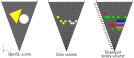
\includegraphics[width=\columnwidth]{images/volumetric/binary_decomposition}
\caption[Volumetric NED: color volume to binary volume decomposition]{Diagram shows the stages of our rendering pipeline: voxelization (see Section~\ref{sec:volumetric:Voxelization}) and binary decomposition (see Section~\ref{sec:volumetric:Decomposition}). For ease of representation, the figure depicts the rendering pipeline for a simple 2-D graphics and 6 bits-per-pixel imagery. Actual implementation uses 3-D graphics and 24 bits-per-pixel imagery. The numbers along the displayed binary volume's frustum indicate the intensity level and color of the RGB LED that illuminates the current binary image.}
%The focal planes are depicted here as equidistant from each other only for ease of representation.}
%Even though the diagram indicates the color volume and binary volume to be in a perspectively shaped volume, the computation is carried out in an orthographic (rectangular) volume. When the display presents the images, it performs an automatic inverse-perspective transformation that corrects for our computations which carried out in the rectangularly shaped volume \kishore{Shorten caption}.}
\label{fig:volumetric:binary_decomposition}
\end{figure}



\subsection{An overview of our rendering pipeline}
The pipeline currently handles only opaque polygons; transparency and other primitives are left to future work. Our rendering pipeline is composed of two steps: (1)  \emph{voxelization}, i.e., the process of converting 3-D polygonal data to a 2-D surface composed of color voxels (3-D equivalent of pixels) that best approximates 3-D polygonal data; and (2) \emph{decomposition} of the color voxels into a series of binary images and corresponding illumination values; these data are used by the display to present a series of single-color binary images to the viewer. 
%Our rendering pipeline can be understood as in three steps: (1) Using 3-D models and scene data, an OpenGL renderer generates an RGB image and a linearized depth map of the current scene at the resolution of the DMD display ($1024 \times 768$).  (2) \emph{voxelization}, i.e., the process of converting graphics primitives from their continuous geometric representations into a set of voxels (3-D equivalent of pixels) that best approximates the graphics primitives; and (3) \emph{decomposition} of the color voxels into a series of binary images and corresponding illumination values; these data are used by the display to present series of binary images to the viewer. \kishore{Mention color}

%We then calculate the color volume by back-projecting the RGB and depth data orthographically. We decompose the color volume to a binary volume on a per-color-voxel basis where the binary voxels corresponding to a color voxel are distributed parallel to the optical axis of the display. The binary images are then displayed on our prototype display, which automatically does a near-inverse perspective projection of the calculated binary images. This is then integrated in the eye or camera to perceive a color volume. 

\subsection{Voxelization: Graphics primitives to 2-D surface}
\label{sec:volumetric:Voxelization}
Using 3-D models and scene data, an OpenGL renderer generates an RGB image and a linearized 16-bit depth map of the current scene at the resolution of the DMD display ($1024 \times 768$). The 16-bit values of the depth map are remapped to the 280 depth values of the focal planes supported by our optical design. This results in a 2-D surface, composed of color voxels, in a $1024 \times 768 \times 280$ volume.

\subsection{Binary Decomposition: Color voxels to binary images}
\label{sec:volumetric:fixed_pipeline}

Our key observation is that the binary representation of a color voxel need not start or end at one of the modulo $3 \times (2^{N_{\text{gray}}} - 1)$ planes as proposed by earlier binary multifocal displays. It need not start or end at one of the modulo $3 \times N_{\text{gray}}$ also, as would be the case for a multifocal NED which displays color image planes using DDS decomposition. Instead, the decomposition of a color voxel to binary voxel can begin and end at arbitrary depths. 

When converting from color volume data to binary images, the intensity and color of each color voxel tell us the binary pattern that represents it, and the depth of the color voxels tells us the center around which the binary pattern should be distributed. The binary voxels that encode the color voxel are distributed along the perspective projection lines that pass through the color voxel's location and the distribution is centered around the color voxel's location. Figure~\ref{fig:volumetric:binary_decomposition} provides a visualization of our rendering pipeline. For ease of representation, Figure~\ref{fig:volumetric:binary_decomposition} depicts the rendering pipeline for equidistant focal planes and for 2-D graphics generating 6 bits-per-pixel imagery. Our implementation handles 24-bits-per-pixel color imagery.


If this decomposition was implemented in an acyclic manner, the number of unique color voxel depths would be $N_b - (3 \times N_{\text{gray}}) + 1$, which is $257$ planes in our case. However, we could implement this decomposition in a cyclic manner, and in this case, the number of unique color voxel depths would be equal to $N_b$, which is 280 in our case. 

Even though we depict in Figure~\ref{fig:volumetric:binary_decomposition} that the decomposition happens in a perspectively shaped volume, it can be implemented as a decomposition on a rectangularly shaped volume. This is indeed the case in our implementation. This is not an issue because when the NED displays the single-color binary images, it does a near-inverse perspective transformation. 

\subsection{Display: Binary images to Retinal image}
The binary images generated are displayed on a DMD in sync with a focus-tunable lens sweeping a sinusoidal or triangular waveform for the optical power of the lens. The single-color binary images displayed by the NED are integrated by the eye to see a color volume. Displaying the binary images in our prototype display is a near inverse-perspective transformation. It is not a perfect inverse-perspective transformation due to the slight change in FoV of images seen over the cycle of the lens (see Figure~\ref{fig:volumetric:graphs}). This near inverse-perspective transformation allows us to perform the transformation of RGB and depth images to color voxels, and the transformation of color voxels to binary voxels in an orthographic space. 

\subsection{Limitations}
\subsubsection{Depth and Spatial resolution}
Conceptually, the minimum non-zero separation in depth between two voxels in our display is $1$ depth plane which averages to $\frac{\text{6.7 diopters}}{\text{280 focal planes}}=\text{0.024 diopters}$. However, because the binary voxels are spread across multiple binary image planes, we should expect to see a blur for the color voxel along the optical axis which could lead to a loss in the depth resolution of the NED. Since each color voxel is represented by multiple binary voxels and the brighter binary voxels are going to be perceived more strongly, we calculate the depth blur as the \emph{weighted} standard deviation of sorted depth values for a moving window of length $3 \times N_{\text{gray}}=24$; this is graphed in the top row of Figure~\ref{fig:volumetric:blur_graphs}. 

Similarly, due to the slightly changing FoV of binary images across the lens cycle (shown in Figure~\ref{fig:volumetric:graphs}), we should expect to see a blur perpendicular to the optical axis which could lead to a loss in the spatial resolution of the NED. This blur is minimum for pixels close to the optical axis and maximum for pixels at the periphery. The maximum angular blur perpendicular to the optical axis is calculated as the standard deviation of FoV values for a moving window of length $3 \times N_{\text{gray}}=24$; this is graphed in the bottom row of Figure~\ref{fig:volumetric:blur_graphs}.

The blur perpendicular to the optical axis can be reduced by performing a calibration to determine the actual FoV of each binary image plane and modifying the color to binary decomposition algorithm to take into account the deformed volume geometry. We did not perform such a calibration process for this chapter. The blur along the optical axis, however, is more fundamental to the display technology. It could be reduced by advanced color volume to binary volume decomposition schemes. 

Previous works have suggested slightly different values for the focal plane separation required for a good multifocal display. Rolland et al.~\cite{Rolland1999dynamic} suggest 0.143 diopters, Akeley et al.~\cite{Akeley2004} design their prototype with image spacings of 0.67 diopters, Liu et al.~\cite{Liu2010systematic} and Watt et al.~\cite{Watt2012Real} suggest 0.6 diopters, and MacKenzie et al.~\cite{MacKenzie2010Accommodation} suggest 1 diopter. As shown in Figure~\ref{fig:volumetric:blur_graphs}, our display has a maximum depth-blur of 0.3 diopters and an average depth-blur of 0.167 diopters. 

\begin{figure}[tb!]
\centering
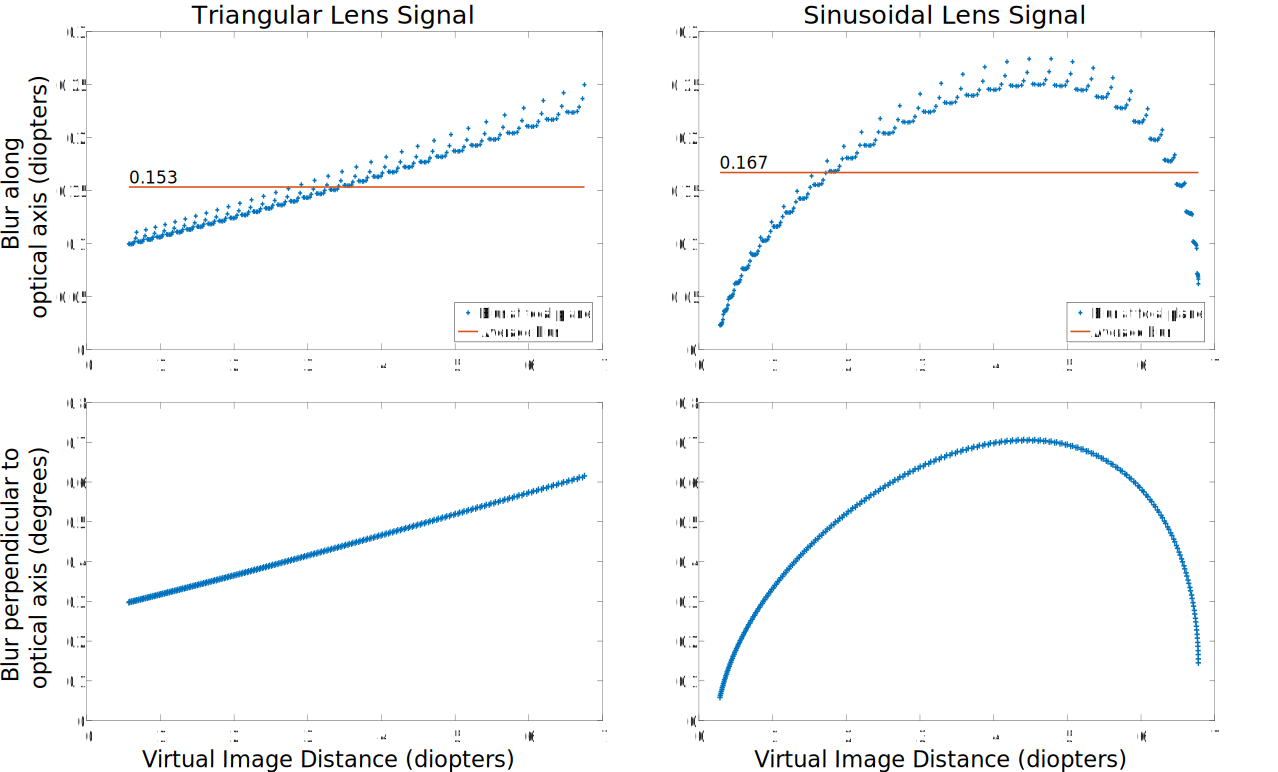
\includegraphics[width=\columnwidth]{images/volumetric/blur_graphs}
\caption[Volumetric NED: Longitudinal and lateral blur of voxels at each depth plane]{\emph{Top row: }Graphs indicate the depth blur for a color voxel at each depth plane and the average depth blur for color voxels of all depth planes. The depth blur arises because the rendering pipeline decomposes each color voxel to multiple single-color binary voxels, which are spread along the perspective projection lines. \emph{Bottom row: } The optics of our NED cause the FoV of the virtual image to slightly change over the lens cycle; this changing FoV is graphed. This creates a blur perpendicular to the optical axis leading to a loss in spatial resolution.}
\label{fig:volumetric:blur_graphs}
\end{figure}
    
    


\subsubsection{Voxel-fighting in a dynamic display implementation}
Here we discuss a minor limitation in extending our proposed offline rendering pipeline to a dynamic display. Observe that to decompose a single color voxel for a 24 bits-per-pixel image, we require 24 binary voxels. In the case of a static display and a cyclic implementation of our decomposition algorithm, this means that a color voxel at, say, the 280th focal plane would be decomposed into binary voxels that range from binary image indices 268 to 12. However, in a dynamic display case, we run into the issue that a new frame is received for each display cycle. 

If the incoming frame information completely replaces the previous frame information, there could be a loss of brightness and bit-depth for the color voxels in the last few focal planes. Alternatively, if we design the NED to start displaying the new frame information only after it finishes displaying the previous frame information, the DMD display's cycle would quickly fall out-of-sync with the lens cycle. With a modified rendering pipeline, for which the framerate of the NED is slightly lower than the frequency of the focus-tunable lens, and very good synchronization of the lens and the DMD, this would not be an issue. Alternatively, we could carry over the information of the last few focal planes of the previous frame to the new frame while giving priority/preference to the new frame's information. 



\section{Static System}
\label{sec:volumetric:static_system}
This chapter presents two rendering pipelines for our display system: (1) One pipeline enables the display to present static volumes. This pipeline is described in this section in a detailed manner. (2) The other pipeline would enable the display to present interactive and dynamically changing volumes. This is still largely under development and this dissertation presents preliminary results in Section \ref{sec:volumetric:rts}.

\subsection{Overview and Software}
To test our ideas, we developed a hardware prototype of a monocular near-eye display and implemented an offline version of our proposed rendering pipeline. The offline rendering pipeline begins with the rendering of a virtual scene using OpenGL/GLSL to generate an RGB image and a linearized 16-bit depth map of the virtual scene. The RGB image and depth map are processed in MATLAB to generate a series of binary images and RGB LED brightness values. The binary images are uploaded to and displayed by the DMD controller, and the RGB LED brightness values are used by a custom RGB LED driver for precise high-speed control over each LED's brightness. An ARM-based microcontroller provides synchronization between the lens, the DMD controller, and the custom RGB LED driver. Below we discuss each hardware component in detail.


\subsection{Hardware}
\paragraph{Focus-tunable Lens} The focus-tunable lens used is the Optotune EL-10-30-TC-VIS. The optical power of the lens is controlled via a manufacturer-provided software and a USB-connected lens driver. The optical power can be set to a static value, or it can be set to follow a rectangular, sinusoidal, or triangular signal for a wide range of frequencies (0.25 Hz to 2000 Hz). For this chapter, all experiments were conducted with the optical power of the lens configured to follow a triangular signal of 60 Hz frequency, and the maximum and minimum lens powers of the triangular signal were approximately 50$m^{-1}$ and 120$m^{-1}$. 


\paragraph{Optics} Other than the focus-tunable lens, we use the manufacturer-provided optical engine of the TI Discovery 4100 Kit (STAR-07 optical module), a Fresnel lens (60mm focal length), and a beamsplitter that allows the display to optically integrate the real world view and the imagery of the virtual scene. 

\paragraph{DMD controller} 
The DMD controller we use is the Texas Instruments (TI) Digital Light Processing (DLP) Discovery 4100 Kit which drives an XGA (1024 x 768) DMD module. The display system is capable of displaying binary images at up to 17241 Hz which would allow 287 binary images to be displayed in each lens cycle. This would need precise synchronization between the lens signal and the DMD controller, which is not afforded by the current implementation. For a more robust system, we display 280 images in each lens cycle and design the system such that the 280 images are guaranteed to be displayed slightly before the beginning of the next lens cycle. 

\paragraph{Custom RGB LED Illuminator}
A PCB mounted RGB LED is controlled using electronics consisting of Digital Analog Converters (DACs), Op-Amps, etc. The board listens for three 16-bit binary codes over Serial Peripheral Interface (SPI) protocol over three parallel buses and sets each color LED to the brightness level corresponding to the received code. The board is capable of illuminating the DMD with a wide range of brightnesses and color combinations. $2^{16}$ levels of intensity are possible for each color LED, and all color LEDs can be driven in parallel. The full-scale rise and fall times of each channel are approximately 500ns; every binary frame can be illuminated at a distinct intensity and color mix. This RGB LED illuminator is the same as the one used in \citet{Lincoln2017scene}; please refer to that chapter for more details. 

\paragraph{PC}
A PC using Intel Xeon E5-2630 2.4 GHz processor with an NVIDIA GeForce GTX 980 running Windows 7 is used to implement an offline version of the proposed rendering pipeline. 

\begin{figure}[tb!]
\centering

\includegraphics[width=\columnwidth]{images/volumetric/blockdiagram-timing}
\caption[Volumetric NED: Overview of static system components and timing relations]{Diagram shows the various hardware components and their timing relations to each other in the display's operational state.}
\label{fig:volumetric:blockdiagram-timing}
\end{figure}


\subsection{Operational detail}
Figure~\ref{fig:volumetric:blockdiagram-timing} gives an overview of the operation of the NED. The binary images are uploaded to the DMD controller using the ALP 4.1 Controller Suite. The DMD controller is configured to advance frames each time it receives a trigger signal from the microcontroller. At the end of the sequence of images, the DMD cycles back to the first image. The frametime of the DMD was set to the minimum possible frametime of 58 $\mu s$.

The lens controller outputs a trigger signal whose rising edges correspond to the beginning of each lens's cycle. The lens operates at a frequency of 60 Hz. The lens' trigger signal is detected by the microcontroller, which then performs $280$ instances of these operations before the next lens' trigger signal: (1) microcontroller outputs a trigger signal to the DMD controller, and (2) microcontroller sends three 16-bit words to the LED controller. Each 16-bit word specifies the brightness of a color LED. The microcontroller ensures that the DMD updates and illumination values are phase-locked to the lens cycle. Figure~\ref{fig:volumetric:setup} shows an image of our display's hardware and the experimental setup. 

\subsubsection{Calibrating phase delay}
In our experience, we've found that there is a phase delay between the lens signal and the displayed image plane depth estimated in Figure~\ref{fig:volumetric:graphs}. This phase delay was calibrated visually by generating a synthetic stack of images in which each image has a single feature (like a cross-hair), but the feature is placed at a different location in each image. By setting the camera lens to nearest focus, it was visually determined that the $180$th image out of the $280$ image stack is in focus, which meant that the lens trigger signal and our system's display of the virtual images are out of phase by $\frac{180 - 140}{280} \times 16.67ms = 2.38 ms$. To correct for this, the binary images uploaded to the DMD controller were cyclically rearranged such that the $180$th binary image is moved to the $140$th index.

\subsection{Future implementation improvements}
The results can be visually improved by performing white-balance correction, gamma curve calibration, and calibrating for the non-uniform frustum as shown in the last row of Figure~\ref{fig:volumetric:graphs}. In our experience, we didn't find the change in FoV to reduce the image quality significantly, but it does make long straight objects slightly curved, especially when the straight objects are places towards the periphery of the display. 


\begin{figure*}[tb!]
\centering
\includegraphics[width=\textwidth]{images/volumetric/results}
\caption[Volumetric NED: results]{View through our volumetric near-eye display where virtual objects are placed among real objects at a range of distances. \emph{Extreme left:} Overhead depiction of scene geometry. Icons to the left of the optical axis correspond to virtual objects, while icons to the right of the optical axis correspond to real objects. \emph{Other images, left to right, in each row:} Photos taken through the display where the focus of the camera is adjusted progressively from near to far. In each row, the only difference between the see-through views is the camera's focus settings - this demonstrates the ability of the display to provide proper focus cues for all virtual pixels simultaneously, allowing the viewer to freely accommodate in the scene without any feedback to the display.}
\label{fig:volumetric:results}
\end{figure*}


\subsection{Results}
\label{sec:volumetric:results}
\paragraph{Cameras}
To record images and videos of the see-through view of the display, cameras that approximate the human eye were placed behind the display (see Figure~\ref{fig:volumetric:setup}) at a distance that approximated the eye relief of a human viewer (2cm away from the beamsplitter). See-through image results presented in this chapter were recorded using a Canon T6i Rebel camera with a Canon 24-70mm f/2.8 lens. See-through video results (in accompanying video submission) were recorded using a Point Grey Chameleon3 camera with a Fujinon 2.8-8mm f/1.2 lens. A 4mm aperture was used in both cameras to emulate the human pupil diameter while collecting results. When using PointGrey cameras, the nearest distance was chosen to be 15cm (6.7 diopters), and when using the DSLR camera, the minimum distance was 20cm (5 diopters) because the lens could not focus closer. 

Our display is capable of presenting virtual imagery closer than 15cm and farther than 4M, but we were constrained by the recording camera (for the minimum distance) and by the lab space (for the farthest distance). Although virtual images closer or farther than what is demonstrated here may not be required for near-eye displays, this may be of use in some other application.

\paragraph{Setup}
Figure~\ref{fig:volumetric:setup} shows the monocular display prototype, the positioning of the camera in place of a viewer's eye and the staged real-world scene consisting of a large poster, and smaller objects such as a Rubik's cube, a wristwatch and a tiny rubber ducky (2cm height). The real world objects are arranged from small to large progressively away from the display approximately along the line of sight of the see-through view. Virtual objects are scaled progressively from small to large away from the display for the virtual objects to subtend approximately the same angle at the camera. 

\paragraph{See-through images}
Figure~\ref{fig:volumetric:results} shows the see-through views of our NED when displaying a virtual scene registered to the staged real-world scene. Even though our RGB LED illuminator can produce high-dynamic range and consequentially very bright virtual imagery~\cite{Lincoln2017scene}, we're currently displaying moderately bright imagery at 24 bits-per-pixel. A black background screen is used to improve visibility and contrast of the virtual objects.

As discussed earlier, the field of view of the virtual image changes during the lens cycle. Ideally, this needs to be calibrated for, but we didn't. Other first order and second order optical aberrations present in all optical systems may also need to be calibrated. Each of these optical aberrations likely varies with depth across the volume. Optical aberrations are observable in our system, e.g., in the second row of Figure~\ref{fig:volumetric:results}, even when focused at the correct depth, the bottom portion of the Jack card is blurred relative to the top. 

To demonstrate that our display shows high-resolution imagery when each binary image is considered individually, Figure~\ref{fig:volumetric:single_plane_images} shows the see-through view when only one of the 280 binary images was encoded with the image of a wire model of a teapot. 

\begin{figure}[htb!]
\centering
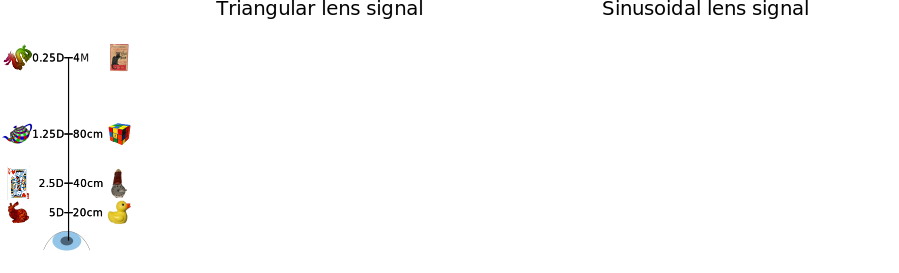
\includegraphics[width=\columnwidth]{images/volumetric/sinusoidal_vs_triangular}
\caption[Volumetric NED: Sinusoidal vs. triangular lens functions]{Images show the see-through view through the display when the optical power of the focus-tunable lens follows a triangular waveform and a sinusoidal waveform. For both these images, the voxelization and color volume to binary volume decomposition was performed assuming a triangular waveform. We don't observe a significant difference in the see-through images.}
\label{fig:volumetric:sinusoidal_vs_triangular}
\end{figure}


Figure~\ref{fig:volumetric:sinusoidal_vs_triangular} shows a comparison between the see-through views when the lens signal follows a triangular and a sinusoidal waveform. This is discussed in Section~\ref{sec:volumetric:sinusoidal_vs_triangular}.


\paragraph{Video results}
A video was recorded as demonstration of this display. This video was submitted as part of this dissertation and is also available publically at this URL: \url{https://www.youtube.com/watch?v=oDcOQ_NotRU}. 
The video results show a larger range of depth (15cm - 4M) compared to the image results (20cm - 4M) because the camera used to record the video was able to focus closer. In these videos, a flicker is seen propagating back and forth through the displayed volume. This flicker is an artifact of the video capture and is not human-visible. The flicker arises because of the slight discrepancy between the display frame time (16.67 ms) and the minimum shutter speed possible on the camera (16.74 ms). The flicker moves back and forth in the volume because the camera samples the whole volume once and a small portion of the volume twice - and because of this, it starts to sample the volume in the subsequent frame from a slightly different starting position of the volume. 



\section{Discussion}
\label{sec:volumetric:discussion}

\subsection{Limitations}
\paragraph{Bulky Optics}
The bulk of the optics is due to the large optical engine of the DLP Discovery 4100 kit, and the tiny aperture of the focus-tunable lens. Other DMD development boards have much smaller optics, and we also note that there is a commercially available AR display that uses a DMD chip~\cite{Dewald2016Avegant}. The small aperture of the focus-tunable lens constrains the optical design and limits the etendue of the system. There are focus-tunable lenses with a wider aperture that could be used, e.g., the focus-tunable lenses presented in \citet{Dunn2017Wide}. If we redesigned the optics and used alternative components, our NED could approach moderate form factor.

\paragraph{Bulky electronic components}
All of the driving electronics (DLP Discovery 4100 kit, custom RGB LED controller, microcontroller) could be reimplemented in a compact ASIC (Application Specific Integrated Circuit) device. 

\subsection{Future Work}
Our near-eye display can emulate some other display technologies, such as multifocal and varifocal displays, and is thus suitable as a versatile platform for user studies. 
The current work could benefit greatly from a compact, wearable, wide-FoV, binocular, and real-time implementation. 
Since the hardware platform and application are similar, this work could be integrated with recent low-latency~\cite{Lincoln2016motion}, and HDR AR~\cite{Lincoln2017scene} displays work. 
This would require combining the volumetric rendering pipeline (presented in this chapter) and the low-latency rendering pipeline (presented in \citet{Lincoln2016motion,Lincoln2017scene,lincoln2017low}).
Another opportunity for research is to investigate if this display can be made entirely independent of eye-tracking requirements. 
Another avenue for future work is to explore adaptive lens functions. 
While this dissertation always oscillates the focal length of the lens according to a sinusoidal or triangular waveform at 60 Hz, the lens is capable of following any arbitrary current waveform. 
While our display demonstrates 280 dioptrically equidistant depth planes, an adaptive lens function can give an adaptive depth distribution of depth planes. 
Uses of such adaptive depth distribution may be foveation in depth, getting high-quality perceptual performance while using fewer depth planes, etc. 

\section{Conclusion}
We have introduced a near-eye volumetric display capable of presenting a large volume over an extended depth-of-field created external to the display's physical volume. We view our system as a hybrid between traditional volumetric displays that create the volume within the confines of the display's physical volume, and view-dependent multifocal near-eye displays. We presented the optical design of our implementation and the rendering pipeline that synthesizes the volume for our display. 
Our main contribution is the idea that color-to-binary volume decomposition can be performed on a per-voxel-basis rather than an image-basis. 
We propose multiple decomposition algorithms and compare them with each other. 
We demonstrate a static display system which shows full-color volumetric display refreshed at 60 Hz and comprising 280 focal planes, each at a unique depth, ranging from 15cm (6.7 diopters) to 4M (0.25 diopters). 
We also demonstrate a dynamic volumetric display system with 8 depth planes. 
One of the key advantages of the proposed volumetric display system is the flexibility of the display system itself. 
It is composed of several components, each of which could be implemented and integrated in different combinations and methods to achieve different results. 
We hope that this system will inspire future research work in near-eye displays to rethink the rendering pipeline. 





\chapter[Varifocal-Occlusion Augmented Reality Display]{Varifocal-Occlusion Augmented Reality Display\footnote{This chapter previously appeared as an article in Transactions on Visualization and Computer Graphics. The original citation is as follows: \bibentry{rathinavel2019varifocal}}}
\label{chapter:varifocal_occlusion_ned}
%\chapter[Varifocal-Occlusion Augmented Reality Display]{Varifocal-Occlusion Augmented Reality Display\raisebox{.3\baselineskip}{\normalsize\footnotemark}}
\chapter[Varifocal-Occlusion Augmented Reality Display]{Varifocal-Occlusion Augmented Reality Display\footnotemark}
\footnotetext{This chapter previously appeared as an article in Transactions on Visualization and Computer Graphics. The original citation is as follows: \bibentry{rathinavel2019varifocal}}
\label{chapter:varifocal_occlusion_ned}

This chapter describes an augmented reality display that presents virtual imagery with support for depth-dependent hard-edge occlusion. 

\section{Introduction}
\label{sec:varifocal_occlusion:introduction}
\begin{figure*}[t]
\centering

\includegraphics[width=0.99\textwidth]{images/varifocal_occlusion/teaser}
%\fbox{\includegraphics[width=0.46\textwidth]{images/prototype}}
\caption[Varifocal-Occlusion NED: teaser]{\textbf{Left of the vertical line:} views through our prototype AR display, which is emulating different AR display technologies for each column. 
The augmented scene is composed of real-world objects (stamp, motorcycle, and gnome) and virtual objects (ring, teapot, and bull). Objects are distributed at different depths: stamp and ring at 30cm, motorcycle and teapot at 100cm, and gnome and bull at 300cm. 
\textit{(Column 1)} Commercially available AR displays: a transparent virtual image is presented at a fixed distance. Important depth cues such as occlusion and accommodation are absent.
\textit{(Column 2)} Varifocal AR displays: virtual image can be moved to different depths, but images are still transparent. 
\textit{(Column 3)} Fixed-focus occlusion-capable AR display: 
Occlusion and virtual image is fixed at a single depth, limiting realism when the user is focused to other depths. Note how all virtual objects, including the nearby ones, are in focus when the camera is focused far, and all virtual objects are defocused when the camera is focused near. 
\textit{(Column 4)} Varifocal occlusion-capable AR displays: virtual and occlusion image plane can be moved to different depths enabling perceptually correct depth cues for occlusion and accommodation. Note how objects at the same depth, e.g., near objects (stamp and ring) or far objects (gnome and bull), are correctly in focus or defocused depending on the focus state of the user/camera.
\textbf{Right of the vertical line:} Comparison of occlusion masks between fixed-focus and varifocal occlusion-capable displays.}
\label{fig:varifocal_occlusion:teaser}
\end{figure*}


Augmented Reality (AR) systems offer unprecedented experiences and are considered a next-generation computing platform. These wearable displays promise to seamlessly augment the physical world around us with digital content, such as information displays or user interfaces. Providing a seamless, perceptually realistic experience, however, requires the display to accurately support all depth cues of the human visual system~\cite{Palmer:1999,Howard:2002}. While current AR displays offer impressive capabilities, they typically do not support the most important depth cue: occlusion~\cite{cutting1995perceiving}.

Providing accurate, i.e., mutually consistent and hard-edge, occlusion between digital and physical objects with optical see-through AR displays is a major challenge. When digital content is located in front of physical objects, the former usually appear semi-transparent and unrealistic (see Fig.~\ref{fig:varifocal_occlusion:teaser}, columns~1 and~2). To adequately render these objects, the light reflected off of the physical object toward the user has to be blocked by the display before impinging on their retina. This occlusion mechanism needs to be programmable to support dynamic scenes and it needs to be perceptually realistic to be effective. The latter implies that occlusion layers are correctly rendered at the distances of the physical objects (see Fig.~\ref{fig:varifocal_occlusion:depth-dependent-occlusion}), allowing for pixel-precise, or hard-edge, control of the transmitted light rays.

Recent proposals on occlusion-capable optical see-through (OST) displays have only partially addressed this challenge. Global dimming~\cite{Mori2018}, for example, is successful in controlling the light transmission of the display but without spatial control. Image-forming systems~\cite{Kiyokawa2003,Cakmakci2004,Gao2012} enable consistent occlusions, but these are only correct at a single distance, severely limiting the image quality at other depths (see Fig.~\ref{fig:varifocal_occlusion:teaser}, column~3) and requiring bulky relay optics. Spatial light modulators (SLMs) for occlusion control can also be used without relay optics~\cite{Itoh2017}, but these will always be out of focus and require additional compensation techniques. Light field-based occlusion technology~\cite{maimone2013general} offers somewhat sharper occlusion control without relay optics. Out-of-focus SLMs~\cite{maimone2013general,Itoh2017} are usually based on liquid crystal displays (LCDs), which introduce diffraction artifacts of the physical world observed in OST displays, thus limiting the perceived image quality.

With this work, we introduce varifocal occlusion-capable optical see-through AR displays. These systems aim at providing a seamless and perceptually realistic experience by providing mutually consistent occlusions over a large depth range (see Fig.~\ref{fig:varifocal_occlusion:teaser}, column~4). Similar to varifocal near-eye displays, our approach uses focus-tunable lenses to dynamically shift the occlusion SLM to a single, but adaptive, optical distance. We envision this approach to operate in a gaze-contingent mode, where an eye tracker determines the distance of the fixated object and both the digital content and the occlusion system are dynamically focused at this distance. 

A unique challenge of varifocal occlusion implemented with focus-tunable optics is precise control of the optical distortion of the physical light. As lenses change their focal power to align the occlusion SLM with different distance of the physical scene, the latter may also be magnified and its perceived distance altered, because the light of the physical scene and the occlusion SLM must share the same optical path. We derive a formal optimization approach and real-time heuristics to drive the proposed system in a perceptually accurate manner, preventing optical distortions of the physical world. 

Specifically, we make the following contributions:
%
\begin{enumerate}
\item We introduce varifocal occlusion as an AR display capability that adaptively changes the focal distance of an occlusion mask to enable hard-edge occlusion over a large depth range. 
\item  We develop an optimization-based optical design approach for our focus-tunable optical system to achieve varifocal occlusion in a perceptually realistic manner without optically distorting the observed scene. 
\item Using insights gained from the optimization approach, we use a ray-transfer matrix approach to derive closed-form solutions for optical designs that allow for varifocal occlusion in real time.
\item We implement a monocular varifocal occlusion-capable AR display and demonstrate improved realism through depth-dependent occlusion.
\end{enumerate}

\begin{figure}[htpb!]
\centering
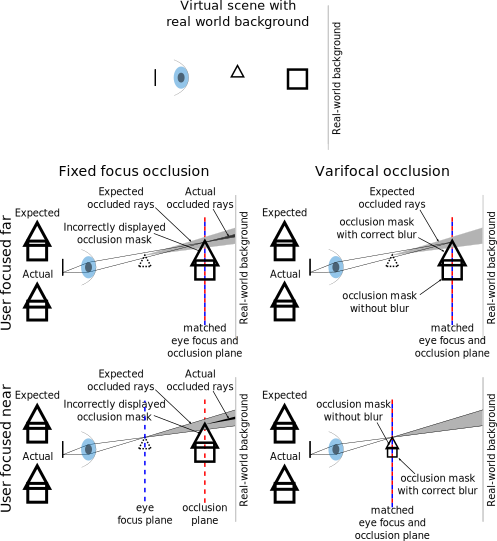
\includegraphics[width=0.9\columnwidth]{images/varifocal_occlusion/depth-dependent-occlusion}
%\fbox{\includegraphics[width=0.46\textwidth]{images/prototype}}
\caption[Varifocal-Occlusion NED: Introducing the concept of depth-dependent occlusion]{\emph{Topmost Row:} A virtual scene composed of one near and one far object placed in front of a real-world background. \emph{Grid of figures:} Comparison of occlusion mechanism only (i.e., ignoring the digital or color image) for fixed-focus and varifocal occlusion displays for the above scene. Dashed blue and red lines indicate the user's focal plane and display's occlusion image plane, respectively. Solid black lines indicate image formation for content placed in the user's focal plane. Images next to the eye show the ``Expected" and ``Actual" images seen by the user. Note that for fixed-focus occlusion, the occlusion plane is always at the far distance which causes the nearby object's occlusion mask to be seen incorrectly always and the far object's occlusion mask to be seen incorrectly when the eye is focused nearby. Varifocal occlusion-capable displays, on the other hand, move the occlusion plane to the user's focal plane and display an occlusion mask for in-focus objects as it is and a perceptually correct occlusion mask for out-of-focus objects by applying a computational blur.}
\label{fig:varifocal_occlusion:depth-dependent-occlusion}
\end{figure}
    



\section{Related Work}
\label{sec:varifocal_occlusion:related}
\renewcommand{\arraystretch}{1.2}
\begin{table}[!htpb]
    \begin{center}
\begin{tabular}{|>{\centering\arraybackslash}m{8cm}|>{\centering\arraybackslash}m{2.0cm}|>{\centering\arraybackslash}m{2.5cm}|}
\hline
Products/Prototypes & AR focus mechanism & Occlusion focus mechanism \\
\hline
HoloLens, Meta2, MagicLeap, etc. & Fixed-focus & None \\
\hline
\citet{Itoh2017} & Fixed-focus & Soft-edge \\
\hline
\citet{Kiyokawa2003}, \citet{Howlett2017}, \citet{Cakmakci2004} & Fixed-focus & Fixed-focus \\
\hline
~\citet{Dunn2017Wide}, \citet{Aksit2017Near} & Varifocal & None \\
\hline
\textbf{\citet{Hamasaki2019}, This chapter} & \textbf{Varifocal} & \textbf{Varifocal} \\
\hline
\end{tabular}
    \end{center}
\caption[Varifocal-Occlusion NED: comparison of focus mechanisms for virtual imagery and occlusion mask in AR displays]{Summary of the type of focus cues that are supported for the virtual imagery and for occlusion by current AR products, previous research prototypes, and this work.}
\label{tab:comparison}
\end{table}


\subsection{Varifocal Near-eye Displays}
\label{sec:varifocal_occlusion:related:varifocal}
Varifocal displays are similar to conventional fixed-focus near-eye displays, but they dynamically adjust the distance of the magnified virtual image. This can be achieved using focus-tunable lenses~\cite{Liu2008Optical,Konrad2016Novel,Johnson:16,Padmanaban2016Optimizing,Laffont:2018,Rathinavel2018}, deformable membranes~\cite{Dunn2017Wide,chakravarthula2018focusar}, or by mechanically actuating optical components~\cite{Shiwa1996proposal,Padmanaban2016Optimizing,Aksit2017Near}. Varifocal displays require eye tracking to determine the distance of the fixated object, to which the display is then focused in a gaze-contingent manner. 


Previous work on varifocal near-eye displays has primarily sought to adjust the virtual image of the digitally displayed content, primarily to mitigate the vergence-accommodation conflict~\cite{kooi2004visual,lambooij2009visual}. %Some recent work extend the concept of varifocal displays to prescription vision correction by re-focusing different depths of the real world into the user's limited accommodation range~\cite{Padmanaban2019Autofocals,chakravarthula2018focusar}. 

In this work, we extend the concept of varifocal displays to the problem of mutually consistent occlusion in AR, where the focus distance of an occlusion SLM is dynamically updated with the goal of improving perceptual realism. 
We discuss optical design strategies and demonstrate a varifocal occlusion-capable AR display that dynamically adjusts the focus of both digital image and occlusion SLM.

\subsection{Occlusion-capable AR displays}

\subsubsection{Projection-based Lighting}

Projection displays can be used to control the lighting of a scene in a spatially varying manner. Using such controlled illumination, mutually consistent occlusions, shading effects, and shadows in projector-based AR systems can be synthesized~\cite{Bimber:2002,bimber2003consistent,maimone2013general,avveduto2017real}.
The primary disadvantages of these systems are that projectors are required for the AR experience, which are not necessarily portable or wearable, and that they may not work in the presence of ambient illumination.
We aim for a fully integrated occlusion-capable AR display that does not require additional projectors.


\subsubsection{Global Dimming} 

Commercial AR displays (e.g., Microsoft HoloLens, Magic Leap) often use a neutral density filter placed on the outside of the display module to reduce ambient light uniformly across the entire field of view.
An adaptive version of global dimming was recently proposed by Mori et al.~\cite{Mori2018}, where the amount of dimming is controlled by a single liquid crystal cell and responsive to its physical environment. While these approaches may be useful in some scenarios, they do not provide spatial control of the occlusion layer.


\subsubsection{Fixed-focus Occlusion} 
\label{sec:varifocal_occlusion:related:fixedfocusOcc}
The physical scene can be focused onto an occlusion SLM which selectively blocks its transmission in a spatially varying manner before it reaches the user's eye. This idea was first proposed by the seminal work of Kiyokawa et al.~\cite{Kiyokawa2000,Kiyokawa2001,Kiyokawa2003}. Improvements of related systems were later demonstrated \cite{Cakmakci2004, Cakmakci2005, Wilson2017, Howlett2017, Wetzstein2010, Gao2012, Gao2013optical}. 

Unfortunately, focusing a scene on an SLM usually requires a bulky optical system, first to focus it to the SLM, then to negate the effect of the first lens, and then to flip the resulting image the right way up. Moreover, as this approach only focuses a single distance of the scene on the occlusion SLM, hard-edge occlusion is only achieved at this fixed focus distance. This limitation is similar to the characteristics of fixed-focus near-eye displays, which has been alleviated by varifocal displays. In this work, we propose an extension of the concept of varifocal displays to occlusion.

Two key challenges for fixed-focus occlusion-capable displays are: (1) to ensure unit magnification of the see-through scene and (2) to ensure zero viewpoint offset between the see-through scene and the real-scene as seen without the display, so that the images of the real-world objects are at the correct distance. Both of these considerations are significantly more challenging for varifocal occlusion displays because unit magnification and zero viewpoint offset needs to be ensured while adjusting the focus of the SLM, which shares the optical path with the physical scene. 

Kiyokawa et al.~\cite{Kiyokawa2003} derive optical design parameters that satisfy unit magnification for all real-world object distances and also propose an interesting geometric configuration of the optical components that make the offset between the real-world objects and their images equal to zero.
Cakmakci et al. \cite{Cakmakci2004} propose a compact optical design that satisfies the magnification requirements, but it does not achieve zero offset between the real viewpoint and the virtual viewpoint; however, the offset is small (5 cm). 
Howlett and Smithwick~\cite{Howlett2017} propose an optical design approach based on ray-transfer matrices to achieve unit magnification and zero viewpoint offset, which is in turn inspired by optical cloaking~\cite{Choi2015}.
We extend the optical design approach based on ray-transfer matrices to varifocal occlusion displays and generalize the theory to asymmetrical optical designs.  

\subsubsection{Soft-edge Occlusion} 

To avoid a bulky optical system, a single LCD can be placed directly in front of the user's eyes~\cite{Wetzstein2010,Itoh2017}. However, due to the fact that the occlusion LCD is out of focus, it always appears blurred. Itoh et al.~\cite{Itoh2017} recently proposed to compensate for this blur by modifying the digitally displayed image.
Such an approach could be interpreted as a hybrid optical see-through and video see-through AR display. 
Calibrating such a system requires extremely precise alignment, and the mismatch in resolution (spatial and angular), latency, brightness, contrast, and color fidelity between the digital display and physical world may contribute to perceived inconsistency and reduced perceptual realism in such a system~\cite{Rolland2000}. 
Maimone et al.~\cite{Maimone2014Pinlight} also used an out-of-focus LCD, where the occlusion mask is calculated as the silhouette of the virtual object. None of these approaches achieves hard-edge occlusion, which severely limits perceptual realism.

\subsubsection{Light Field Occlusion}
Maimone and Fuchs~\cite{maimone2013general} propose a 4D light field occlusion mask using stacked LCD layers placed out of focus in front of the eye, where the occluding patterns are calculated by light field factorization algorithms~\cite{Lanman2010, Wetzstein2012}. 
The advantage of light field occlusion is that depth-dependent occlusion can be presented for virtual content at different depths simultaneously in a compact form factor. 
In practice, see-through LCDs mounted close to the eye are light inefficient and result in significant diffraction artifacts, which are due to the electronic components in each pixel as well as the wiring of the display panel. This effect significantly degrades the observed image quality of any soft-edge or light field occlusion system. 

Another approach for light field occlusion is presented in \cite{Yamaguchi2016} using concepts of integral imaging systems. This system has a very narrow field of view (4.3 degrees) and is fundamentally limited by the spatio-angular resolution tradeoff as well as diffraction.

As opposed to any of these methods, the proposed varifocal occlusion approach achieves hard-edge occlusion at varying distances in the scene at high resolution, with better light efficiency, and using technology components that make it easily compatible with emerging varifocal near-eye display. 

\subsubsection{Varifocal Occlusion}
Concurrently and independently of our work, Hamasaki and Itoh~\cite{Hamasaki2019} also developed a strategy for a varifocal occlusion-capable AR display. Unlike our approach that builds on focus-tunable optics to dynamically adjust the depth of the occlusion layer, their approach requires mechanical motion of the occlusion SLM. Each approach has certain benefits and limitations. For example, robust calibration of the mechanically moving parts in their approach can be challenging, especially in a wearable display form factor. Our approach, on the other hand, requires focus-tunable optics, such as liquid lenses or Alvarez lenses (see Sec.~\ref{sec:varifocal_occlusion:related:varifocal}).

\subsection{Consistent Colors, Shading, and Shadows in AR}
Spatial AR systems and optical see-through AR display often aim at providing radiometrically consistent, color-corrected or even color-stylized imagery~\cite{Bimber:2008,Wetzstein2010,Langlotz:2016,Langlotz2018,Itoh2019}. All of these approaches are successful in enhancing the viewing experience in AR, but none of them tackle the problem of mutually consistent occlusions in optical see-through AR displays.


\section{Optical Design}
\label{sec:varifocal_occlusion:design}
\begin{figure*}
\centering
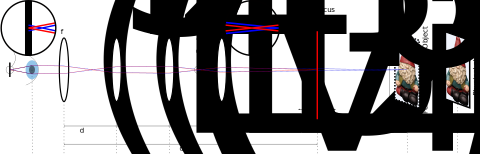
\includegraphics[width=0.89\textwidth]{images/varifocal_occlusion/unfolded}
%\fbox{\includegraphics[width=0.46\textwidth]{images/prototype}}
\caption[Varifocal-Occlusion: unfolded optics]{Illustration of the unfolded optical path of a 4-lens system for image-forming occlusion-capable AR displays. With a varifocal display, the distance of virtual image and occlusion mask matches the user's focus distance, indicated by the thick vertical red line. Red and blue lines going from points in the scene through the optics onto the retina indicate ray diagrams for the image formation of the virtual/occlusion image and for physical objects, respectively. Enlarged inset at the occlusion SLM shows that the physical world at the user's focus plane is brought into focus at the SLM where portions of the real world can be occluded. Enlarged inset at the retina shows that the same rays (red) that are in-focus at the occlusion SLM are also in-focus at the retina -- this property is utilized to also depict a perceptually correct occlusion mask for out-of-focus virtual objects by applying a computational blur. Finally, the image of real-world objects seen through the display should ideally have the same magnification and distances from the eye as compared to seeing the real world without the display, i.e. $\frac{h_i}{h_o}=1$ and $e=0$. In our implementation, we are able to match the magnification, but not the distance.}
\label{fig:varifocal_occlusion:unfolded}
\end{figure*}

Our goal is to design a varifocal occlusion-capable OST AR display that satisfies several key requirements. These include 
%
\begin{enumerate}
    \item The virtual image of the occlusion SLM, i.e. the occlusion mask, and the digital image should be optically placed together in the scene and their distance be dynamically adjustable.
    \item The lateral and longitudinal magnification of the physical scene seen through the display should be equal to one, such that the experience is similar to viewing the scene without any optical elements.
    \item No mechanical motion should be introduced to any component (lenses, SLM, etc.) to adjust the distance of its virtual image. Instead, the virtual image should be moved by changing the focal powers of the employed lenses.
\end{enumerate}
%

In the following, we first provide an overview of the optical design we consider, introduce a ray-transfer matrix analysis of prior work on fixed-focus occlusion-capable AR displays (see Sec.~\ref{sec:varifocal_occlusion:related:fixedfocusOcc}), and  finally introduce our focus-tunable varifocal occlusion approach.

\paragraph{\textbf{Overview of the optical design}}
We consider an optical design composed of four lenses (see Fig.~\ref{fig:varifocal_occlusion:unfolded}), whose respective functions are: The first lens brings the real world at a particular depth into focus at the SLM. This image is always flipped, similar to how the image of the real world that is formed on our retina inside our eyes is always flipped. The next two lenses re-invert the in-focus image at the SLM, similar to a 4f system. The last lens finally places the image back into the appropriate depth for comfortable viewing. Let us denote these lenses by $L_1,L_2,L_3,L_4$ (see Fig.~\ref{fig:varifocal_occlusion:unfolded}).

The occlusion SLM can be placed in any of the image planes of the optical system. There are two locations for this, one is between $L_1$ and $L_2$ and the other is between $L_3$ and $L_4$. We place the occlusion SLM between $L_1$ and $L_2$ because it simplifies Eq.~\eqref{eq:closed_form_f_1}. The digital image SLM can also be placed in any of the image planes of the optical system. We choose to place it between $L_1$ and $L_2$ because in this case, we can treat both the occlusion SLM and the virtual SLM to be optically equivalent and derive just one set of conditions for both of them.

%%%%%%%%%%%%%%%%%%%%%%%%%%%%%%%%%%%%%%%%%%%%%%%%%%%%%%%%%%%%%%%%%%%%%%%%%%%%%%%%%%%%%%%%%%%%%%%%%%
\subsection{Modeling Fixed-focus Occlusion Masks}
\label{sec:optical_design_fixed_focus}

%In this subsection, we discuss previous approaches to display an occlusion mask at a fixed depth. Such systems satisfy the first three requirements listed earlier. We restrict discussion of previous works to the image-forming occlusion type. 

%\kishore{Move to related work}
%Kiyokawa et al. \cite{Kiyokawa2003} derive optical design parameters that satisfy unit magnification for all real-world object distances and propose an interesting geometric configuration of the optical components that make the offset between the real world objects and images equal to zero.
%Cakmakci et al. \cite{Cakmakci2004} propose a compact optical design that satisfies the magnification requirements. 
%Cakmakci et al.'s \cite{Cakmakci2004} design does not guarantee that the offset between the real viewpoint and the virtual viewpoint should be zero; however, the offset is small (5 cm). 
%The design approach in these papers was primarily based on algebraic analysis of the Gaussian form of the thin lens equation to guarantee that the magnification is one, and coming up with an interesting folded optics design to ensure that the real viewpoint and virtual viewpoint are coincident, if possible. 

%Other previous papers propose a more general approach based on ray-transfer matrix analysis, summarized below.

%\subsubsection{Ray-transfer matrix}

The light transport through optical components can be modeled using ray-transfer matrices. In this approach, a light ray is represented by a column vector composed of lateral distance ($x$) and angle of propagation ($\theta$) with respect to the optical axis. 
The propagation of paraxial light rays through an optical component is modeled as the multiplication of the ray vector with a $2 \times 2$ ray-transfer matrix. Ray-transfer matrices are known for standard optical components, e.g. let us denote the ray-transfer matrix for a lens with focal length $f$ by $\mathbf{M}$ and the ray-transfer matrix for free-space propagation with a distance $d$ by $\mathbf{S}$. Then, $\mathbf{M}$ and $\mathbf{S}$ are given by:

%
\begin{equation}
\mathbf{M} = 
\begin{bmatrix}
1 & 0 \\
-\frac{1}{f} & 1 
\end{bmatrix},
\quad \quad
\mathbf{S} = 
\begin{bmatrix}
1 & d \\
0 & 1 
\end{bmatrix}.
\end{equation}
%
The composite ray transfer matrix that models the propagation of light rays through a series of optical components is simply the multiplication of the various individual ray transfer matrices of each optical component. 

For our optical design (Fig.~\ref{fig:varifocal_occlusion:unfolded}), the composite ray transfer matrix is represented as:
%
\begin{equation}
\mathbf{T} = \mathbf{M}_4 \mathbf{S}_{(L_3,L_4)} \mathbf{M}_3 \mathbf{S}_{(L_2,L_3)} \mathbf{M}_2 \mathbf{S}_{(L_1,L_2)} \mathbf{M}_1,
\label{eq:static_general}
\end{equation}
%
where $\mathbf{M}_i$ is the ray-transfer matrix describing $L_i$ and $\mathbf{S}_{(L_i,L_j)}$ describes the free-space propagation between lenses $L_i$ and $L_j$.

The above linear system of equations is composed of four equations and seven unknowns (four unknown focal lengths and three unknown distances). This is an ill-posed inverse problem. Instead of attempting to solve it directly, previous works relied on symmetry constraints, such that $f_1 = f_4$, $f_2 = f_3$, and $d_{(L_1,L_2)} = d_{(L_3,L_4)}$.

%which makes the composite ray transfer matrix:
%
%\begin{equation}
%T = M_1 S_{(1,2)} M_2 S_{(2,3)} M_2 S_{(1,2)} M_1.
%\label{eq:static_symmetric}
%\end{equation}
%
%This system of linear equations has four unknowns and is solvable analytically.

Previous works have explored mainly two choices for the composite ray transfer matrix. 

{\bf Shifted Perspective. $\,\,$}
In this configuration, the virtual viewpoint is shifted to the front of the optical system. In other words, the first lens and the last lens form conjugate aperture planes. Another way to think of it is that the light field entering the optical system and the light field exiting the optical system are equivalent. Mathematically, this condition represents $\mathbf{T} = \mathbf{I}$, where $\mathbf{I}$ is the $2 \times 2$ identity matrix. Some of the earlier prototypes of Kiyokawa et al.~\cite{Kiyokawa2000,Kiyokawa2001} and Cakmakci et al.~\cite{Cakmakci2004} had a shifted perspective. 

{\bf Correct Perspective. $\,\,$}
In this configuration, a user looking through the optical system should see the exact same image of a physical scene behind it as if the optical system was absent. There is no shift in the viewpoint. Kiyokawa et al.~\cite{Kiyokawa2003} proposed a folded optics design for achieving correct perspective. This condition was analyzed formally with ray-transfer matrix equations for the first time in the context of optical cloaking~\cite{Choi2015} and later applied to the problem of occlusion in AR displays~\cite{Howlett2017}. Mathematically, this is represented via the ray-transfer matrix $\mathbf{T} = \mathbf{S}_{(L_1,L_4)}$.

%\paragraph{Choosing between the two constraints}
While an OST AR display should ideally be made to satisfy the correct perspective constraint, the disadvantage in doing so is that the field of view of the optical system is much smaller, being at most equal to the field of view seen through the first lens' aperture from a viewing distance of the length of the optical system. This limitation is exacerbated in our implementation by the small aperture (1 cm) of our focus-tunable lenses. For this reason, we design and implement an optical system that satisfies the shifted-perspective constraint. 

%\subsubsection{Previous approach applied to varifocal occlusion}
%The optical design solution which was calculated using ray-transfer matrix approach in the previous works will extend to a varifocal occlusion display trivially, but will require all the fixed-focal length lenses to be replaced by focus-tunable lenses and will require that the lenses be movable dynamically. Mathematically, having all lenses and distances as dynamic parameters, with the symmetry constraints of $f_1^{(t)} = f_4^{(t)}$, $f_2^{(t)} = f_3^{(t)}$, and $d_{(L_1,L_2)}^{(t)} = d_{(L_3,L_4)}^{(t)}$, the ray-transfer matrix would be:
%\begin{equation}
%    T = M_1^{(t)} S_{(1,2)}^{(t)} M_2^{(t)} S_{(2,3)}^{(t)} M_2^{(t)} S_{(1,2)}^{(t)} M_1^{(t)},
%\end{equation}
%where we denote dynamic parameters with the superscript $^{(t)}$.
%This would result in an overly complicated system. Below, we discuss our approach.


%%%%%%%%%%%%%%%%%%%%%%%%%%%%%%%%%%%%%%%%%%%%%%%%%%%%%%%%%%%%%%%%%%%%%%%%%%%%%%%%%%%%%%%%%%%%%%%%%%
\subsection{Modeling Varifocal Occlusion Masks}
\label{sec:optical_design:varifocal_occlusion_mask}

Consider the general system of linear equations for image-forming occlusion optical designs (Eq.~\eqref{eq:static_general}). Recall that solving this is not possible by simply analyzing the ray-transfer matrix equations because there are more unknowns than equations. Our approach is to apply an optimization approach to this problem. Gaining some insights from the optimization approach, we then revisit the ray-transfer matrices approach to derive closed-form solutions.

Both our approaches aim to satisfy these requirements:
\begin{enumerate}
   \item  
    the virtual image should be placed at a desired (but movable) distance.
    \item 
    the magnification of the see-through image of the real-world should be unity irrespective of the virtual image plane distance. 
\end{enumerate}

\subsubsection{Optimization approach}
\label{sec:optical_design_optimization}
The optimization approach needs to calculate the set of focal lengths that minimize the error in the magnification of the see-through view and the error in the virtual/occlusion image plane's depth.

To do this, we define an image formation model for OST occlusion-capable displays, a cost function for the errors, and apply known methods to minimize the error iteratively. We start off by assuming that all lenses are focus-tunable lenses.

\paragraph{\textbf{Image Formation}}
The image formation for the virtual and real-world is modeled by successive application of the Gaussian thin lens equations:

\begin{equation}
i = \frac{o f}{o - f},
\label{eq:gaussian_thin_lens_equation}
\end{equation}
where $i$ is the image distance, $o$ is the object distance, and $f$ is the focal length of the lens.

For an optical system composed of multiple lenses, the object of the subsequent lens ($L_{j+1}$) is the image of the previous lens ($L_{j}$). So, the object distance for $L_{j+1}$ is: $o_{j+1} = d_{(L_j, L_{j+1})} - i_j$.

\paragraph{\textbf{Occlusion and Virtual Image Formation}}
For the occlusion and virtual image, the objects are the occlusion and virtual SLMs which are optically placed together by design. Only the lenses between these SLMs and the eye ($L_2,L_3,L_4$) contribute to the virtual/occlusion image formation. So, the object distance ($d_{(\text{SLM},L_2)}$) is propagated through lenses $L_2$, $L_3$, and $L_4$, to obtain the distance to the perceived occlusion/virtual image plane from lens 4 ($d_{(\text{vip},L_4)}$). Let us denote this image formation function by:
\begin{equation}
[d_{(\text{vip},L_4)}] = I_V(f_2, f_3, f_4, d_{(\text{SLM}, L_2)}, d_{(L_2,L_3)}, d_{(L_3,L_4)}),
\label{eq:optimization_virtual_image_formation}
\end{equation}
where $I_V$ is composed of the successive application of Eq.~\eqref{eq:gaussian_thin_lens_equation}, beginning with
\begin{equation}
i_2 = \frac{d_{(\text{SLM},L_2)} f_2}{d_{(\text{SLM},L_2)}-f_2},
\quad \quad
o_{3} = d_{(L_2,L_3)} - i_2,
\end{equation}
and ending with:
\begin{equation}
d_{(\text{vip},L_4)} = \frac{o_4 f_4}{o_4 - f_4}.
\end{equation}

\paragraph{\textbf{See-Through Image Formation}}
For the real-world, we first discretize the real-world into $N$ real-world depth planes, where the number $N$ is chosen such that the system samples the real-world denser than the human eye's depth-of-field which has been measured to be $0.3$ diopters~\cite{Campbell1957,Watt2005}. So, for a display whose nearest and farthest depth planes are at $D_{(R_{\text{near}}, L_1)}$ diopters and $D_{(R_{\text{far}}, L_1)}$ diopters respectively, the minimum number of discretized real-world depth planes should be:

\begin{equation}
N > \frac{D_{(R_{\text{near}},L_1)} - D_{(R_{\text{far}},L_1)}}{0.3}.
\label{eq:optimization:number_of_planes}
\end{equation}

Each real-world depth ($d_{(R_j,L_1)}$) is propagated through lenses $L_1,L_2,L_3,L_4$ from which we get the see-through image depth from $L_4$ ($d_{(V_j,L_4)}$):
\begin{align}
&[d_{(V_1,L_4)}, d_{(V_2,L_4)},...,d_{(V_N,L_4)}] = \nonumber\\
&I_R(f_1, f_2, f_3, f_4, d_{(L_1,L_2)}, d_{(L_2,L_3)}, d_{(L_3,L_4)}, d_{(R_1,L_1)},d_{(R_2,L_1)},...,d_{(R_N,L_1)}),
\label{eq:optimization_real_image_formation}
\end{align}
where $I_R$ is a successive application of Eq.~\eqref{eq:gaussian_thin_lens_equation} for each discretized real-world depth plane beginning with:
\begin{equation}
i_1 = \frac{d_{(R_j,L_1)} f_1}{d_{(R_j,L_1)}-f_1},
\quad \quad
o_{2} = d_{(L_1,L_2)} - i_1,
\end{equation}
and ending with:
\begin{equation}
d_{(V_j,L_4)} = \frac{o_4 f_4}{o_4 - f_4}.
\end{equation}

\paragraph{\textbf{Error function}}
The error associated with the occlusion/virtual image is the difference between desired occlusion/virtual image plane depth ($d_{in}$) and actual occlusion/virtual image plane depth ($d_{(\text{vip},L_4)}$) calculated as: $d_{in} - d_{(\text{vip},L_4)}$.

The error associated with the magnification of the physical scene is the difference between one and the magnification of the see-through image, where magnification is calculated as $m = -\frac{\text{image distance}}{\text{object distance}}$. However, in calculating the magnification, we need to be careful about what we consider as the object distance: Recall that in the see-through image formation function (Eq.~\eqref{eq:optimization_real_image_formation}), we've defined the real-world object distances with respect to the first lens ($d_{(R_j, L_1)}$), whereas the final image distance is calculated with respect to the last lens ($d_{(V_j, L_4)}$). This discrepancy is alright when the optical system is designed to satisfy the shifted-perspective constraint. However, for the correct-perspective constraint, the object distance should be modified to $d_{(R_j,L_1)}+d_{(L_1,L_4)}$. For our display, where the correct object distance is $d_{(R_j,L_1)}$ and the magnification is given by $m_j=-\frac{d_{(V_j,L_4)}}{d_{(R_j,L_1)}}$

The combined error vector is given below:
\begin{equation}
    E = 
    \begin{bmatrix} 
    d_{\text{in}} - d_{(\text{vip},L_4)}\\ 
    1 - m_1\\ 
    1 - m_2\\ 
    ...\\ 
    1 - m_N\\ 
    \end{bmatrix}.
    \label{eq:optimization_error}
\end{equation}

The optimization problem is to find a set of focal lengths ($f_1,f_2,f_3,f_4$) that minimize the above error:
\begin{equation}
\argmin_{f_1,f_2,f_3,f_4} ||E||^2.
\end{equation}

Our implementation of this indicates that the set of focal lengths that minimizes the above error function always has a fixed $f_2$ and $f_3$. 

Unfortunately, the execution time of this optimization is not real-time. We could calculate the dynamic values of $f_1$ and $f_4$ for different occlusion mask distances and use the calculated values in a look-up table to get real-time performance. Alternatively, we could use the new information that a fixed $f_2$ and $f_3$ can satisfy all the requirements to calculate closed-form solutions, as discussed below.

\subsubsection{Closed-form solutions}
\label{sec:optical_design_closed_form}

Consider the same 4-lens optical design for a varifocal occlusion-capable display composed of the following parameters: $f_1^{(t)}, f_2, f_3, f_4^{(t)}, d_{(L_1,L_2)}, d_{(L_2,L_3)}, d_{(L_3,L_4)}, d_{(\text{SLM},L_1)}$, where the superscript $\cdot ^{(t)}$ indicates a dynamically changing parameter. 


Using the Gaussian thin lens equation (Eq.~\eqref{eq:gaussian_thin_lens_equation}), $f_1^{(t)}$ is calculated based on the desired virtual image plane distance ($d_{(\text{vip},L_1)}^{(t)}$) and the distance between $L_1$ and the occluding SLM ($d_{(\text{SLM},L_1)}$):
\begin{equation}
    f_1^{(t)} = \frac{d_{(\text{vip},L_1)}^{(t)} d_{(\text{SLM},L_1)} }{d_{(\text{vip},L_1)}^{(t)} + d_{(\text{SLM},L_1)} }.
    \label{eq:closed_form_f_1}
\end{equation}

Solving for the rest of the parameters needs an analysis of the ray-transfer matrix equation. To satisfy the shifted-perspective condition, the ray-transfer matrix needs to satisfy:
\begin{equation}
    \mathbf{I} = \mathbf{M}_4^{(t)} \mathbf{S}_{(L_3,L_4)} \mathbf{M}_3 \mathbf{S}_{(L_2,L_3)} \mathbf{M}_2 \mathbf{S}_{(L_1,L_2)} \mathbf{M}_1^{(t)}.
    \label{eq:II_eq_TA}
\end{equation}
Finding optical parameter values that satisfy the above equation automatically ensures that the requirements listed in the beginning of Sec.~\ref{sec:optical_design:varifocal_occlusion_mask} will be satisfied. Since we have learned from our optimization experiments that solutions exists where $L_2$ and $L_3$ are fixed-focal length lenses, we solve Eq.~\eqref{eq:II_eq_TA} for $\mathbf{M}_4^{(t)}$ and analyze the conditions that ensure that the constants of matrix $\mathbf{M}_4^{(t)}$ (i.e., the ones and zero of $\mathbf{M}_4^{(t)}$) are their appropriate values: 

\begin{equation}
\mathbf{M}_4^{(t)} \overset{a}{=} 
\begin{bmatrix}
\frac{1 + BC}{\frac{C}{f_1^{(t)}} + A} & C \\
B & \frac{C}{f_1^{(t)}} + A
\end{bmatrix}
\overset{b}{=}
\begin{bmatrix}
1 & 0 \\
-\frac{1}{f_4^{(t)}} & 1 
\end{bmatrix},
\label{eq:closed_form_I}
\end{equation}
where $\overset{a}{=}$ is obtained by solving Eq.~\eqref{eq:II_eq_TA} for $\mathbf{M}_4^{(t)}$ and $\overset{b}{=}$  is obtained because $\mathbf{M}_4^{(t)}$ should have the ray-trasfer matrix for a lens, and where $A$, $B$, $C$ are the following:
% \begin{flalign}
% &A = 1 - \frac{d_{(L_3,L_4)} + d_{(L_2,L_3)} \left(1 - \frac{d_{(L_3,L_4)}}{f_{3}}\right)}{f_{2}} - \frac{d_{(L_3,L_4)}}{f_{3}}, \label{eq:shifted_perspective_A} \\ 
% &B = \frac{1 - \frac{d_{(L_2,L_3)}}{f_{3}} - d_{(L_1,L_2)} \left(\frac{1 - \frac{d_{(L_2,L_3)}}{f_{3}}}{f_{2}} + \frac{1}{f_{3}}\right)}{f_1^{(t)}} + \frac{1 - \frac{d_{(L_2,L_3)}}{f_{3}}}{f_{2}} + \frac{1}{f_{3}}, \label{eq:shifted_perspective_B} \\
% &C = d_{(L_2,L_3)} \left(1 - \frac{d_{(L_3,L_4)}}{f_{3}}\right) + d_{(L_3,L_4)} + d_{(L_1,L_2)}A. \label{eq:shifted_perspective_C}
% \end{flalign}

\begin{equation}
    A = 1 - \frac{d_{(L_3,L_4)} + d_{(L_2,L_3)} \left(1 - \frac{d_{(L_3,L_4)}}{f_{3}}\right)}{f_{2}} - \frac{d_{(L_3,L_4)}}{f_{3}}, \label{eq:shifted_perspective_A}
\end{equation}

\begin{equation}
    B = \frac{1 - \frac{d_{(L_2,L_3)}}{f_{3}} - d_{(L_1,L_2)} \left(\frac{1 - \frac{d_{(L_2,L_3)}}{f_{3}}}{f_{2}} + \frac{1}{f_{3}}\right)}{f_1^{(t)}} + \frac{1 - \frac{d_{(L_2,L_3)}}{f_{3}}}{f_{2}} + \frac{1}{f_{3}},
    \label{eq:shifted_perspective_B}
\end{equation}

\begin{equation}
    C = d_{(L_2,L_3)} \left(1 - \frac{d_{(L_3,L_4)}}{f_{3}}\right) + d_{(L_3,L_4)} + d_{(L_1,L_2)}A.
    \label{eq:shifted_perspective_C}
\end{equation}

From Eq.~\eqref{eq:closed_form_I}, we can infer that $C=0$, and thereby, we can derive that $A=1$ by substituting $C=0$ in:
\begin{equation}
    1 = \frac{C}{f_1^{(t)}} + A.
\end{equation}

Re-arranging Eq.~\eqref{eq:shifted_perspective_A} by substituting $A = 1$:
\begin{equation}
    - \frac{f_2}{f_3} = 1 + \frac{d_{(L_2,L_3)}}{d_{(L_3,L_4)}}\left( 1 - \frac{d_{(L_3,L_4)}}{f_3}\right).
\end{equation}

Re-arranging Eq.~\eqref{eq:shifted_perspective_C} by substituting $C = 0$ and $A = 1$:
\begin{equation}
   - \frac{d_{(L_1,L_2)}}{d_{(L_3,L_4)}} = 1 + \frac{d_{(L_2,L_3)}}{d_{(L_3,L_4)}}\left( 1 - \frac{d_{(L_3,L_4)}}{f_{3}}\right).
\end{equation}

This gives us the condition that:
\begin{equation}
\frac{d_{(L_1,L_2)}}{d_{(L_3,L_4)}} = \frac{f_2}{f_3}.
\label{eq:closed_form_d_f_relation}
\end{equation}

$d_{(L_2,L_3)}$ can be derived by re-arranging Eq.~\eqref{eq:shifted_perspective_C} and substituting $d_{(L_1,L_2)}=\frac{d_{(L_3,L_4)}f_2}{f_3}$, $A = 1$, and $C=0$:
\begin{align}
    - \frac{f_2d_{(L_3,L_4)}}{f_3} &= d_{(L_3,L_4)} + d_{(L_2,L_3)}\left(1 - \frac{d_{(L_3,L_4)}}{f_3} \right)\nonumber\\
    \implies d_{(L_2,L_3)} &= \frac{d_{(L_3,L_4)}\left(1 + \frac{f_2}{f_3} \right)}{\frac{d_{(L_3,L_4)}}{f_3} - 1}.
    \label{eq:closed_form_d_23}
\end{align}

$d_{(L_2,L_3)}$ has to be positive. This gives us an improved version of the condition in Eq.~\eqref{eq:closed_form_d_f_relation}:
\begin{equation}
    \frac{d_{(L_3,L_4)}}{f_3} = \frac{d_{(L_1,L_2)}}{f_2} > 1.
    \label{eq:closed_form_d_f_relation_2}
\end{equation}

$f_4^{(t)}$ is primary calculated from Equations~\eqref{eq:closed_form_I} and \eqref{eq:shifted_perspective_B}:
\begin{equation}
    f_4{^{(t)}} = -\frac{1}{B}.
    \label{eq:closed_form_f_4}
\end{equation}

\paragraph{\textbf{Summary}}
Here are steps that can be taken to arrive at the static parameters of the optical design:
\begin{enumerate}
    \item Using Eq.~\eqref{eq:closed_form_d_f_relation_2}, choose any three among $d_{(L_1,L_2)}, d_{(L_3,L_4)}, f_2, f_3$ and calculate for the fourth parameter. This choice can be based on the available fixed-focus lenses for $f_2$ and $f_3$ or based on constraints placed upon $d_{(L_1,L_2)}$ and $d_{(L_3,L_4)}$ by the hardware prototype. Although $d_{(\text{SLM},L_1)}$ doesn't feature in any of the conditions that we've derived, it should also be considered carefully in this step because it influences $d_{(L_1,L_2)}$ in that $d_{(L_1,L_2)} > d_{(\text{SLM},L_1)}$. 
    \item $d_{(L_2,L_3)}$ can now be calculated using Eq.~\eqref{eq:closed_form_d_23}.
\end{enumerate}


During the operation of the display, the dynamic parameters ($f_1^{(t)}$ and $f_4^{(t)}$) are calculated using Equations~\eqref{eq:closed_form_f_1} and \eqref{eq:closed_form_f_4} which are in turn dependent on only one dynamic value which is the virtual image distance ($d_{(\text{vip},L_1)}^{(t)}$). 

Again, these equations ensure Eq.~\eqref{eq:II_eq_TA} which means that the see-through image of the real world would have unit magnification, although with a longitudinal shift which is equal to the length of the optical system from $L_1$ to $L_4$.



\section{Implementation}
\label{sec:varifocal_occlusion:implementation}
\begin{figure}[t]
\centering
\includegraphics[width=0.65\columnwidth]{images/varifocal_occlusion/prototype}
%\fbox{\includegraphics[width=0.46\textwidth]{images/prototype}}
\caption[varifocal-Occlusion NED: Benchtop prototype and staged real-world scene for capturing results]{\textit{(A)} Photo of our varifocal occlusion-capable AR display \textit{(B)} Optical design of the prototype. Static design parameters are denoted in green. Propagation of real-world light through the system is depicted with red arrows. Propagation of the virtual image is depicted with blue arrows. The arrows are only representative of the general direction of propagation and do not depict the exact path taken by the light rays. \textit{(C)} Photo of lab set-up which shows the prototype and the three real objects: stamp at 30cm, motorcycle at 100cm, and gnome at 300cm.}
\label{fig:varifocal_occlusion:prototype}
\end{figure}

We demonstrate varifocal occlusion with a monocular benchtop prototype (see Fig.~\ref{fig:varifocal_occlusion:prototype} (A)). Optical design details and components details are discussed in the following.

{\bf Optical Design. $\,\,$} To minimize distortion and chromatic aberrations in the prototype, all fixed-focus lenses ($L_2$, $L_3$) in our prototype are Nikon Nikkor 35-mm f/2 camera lenses. We use a 30-mm cage polarizing beamsplitter cube (ThorLabs CCM1-PBS251) to combine the real-world view after occlusion and the digital image. This design choice and the bulkiness of the Nikon imaging lenses constrains $d_{(L_1,L_2)}$ to a minimum of 10~cm. With this choice of parameters, and for an augmented scene whose minimum and maximum occlusion/virtual image plane depths are 30~cm and 300~cm, respectively, we obtain $f_1^{(t)}$ to lie in the range 25--28.5 diopters and $f_4^{(t)}$ in the range 2.64--5.67 diopters by using our closed-form solutions (Sec.~\ref{sec:optical_design_closed_form}).
However, neither of these ranges of optical powers is directly supported by the focus-tunable lenses. The focus-tunable lenses in our prototype are Optotune EL-10-30-TC whose focal range is 8.3--20 diopters and Optotune EL-10-30-C whose focal range is 5--10 diopters. 

Additional offset lenses are necessary to bring the operating range of optical powers into the supported range. The combined lens power ($D_{\text{combined}}$) of a focus-tunable lens ($D_{\text{tunable}}^{(t)}$) and an offset lens ($D_{\text{offset}}$) is theoretically $D_{\text{combined}} = D_{\text{offset}} + D_{\text{tunable}}^{(t)}$. In practice, however, we cannot place the offset lens exactly on top of the focus-tunable lens, so it is necessary to modify the composite ray-transfer matrix equations to additionally model the free-space propagation between offset and focus-tunable lenses. 

Adding offset lenses changes the composite ray-transfer matrix and solving the equations analytically is tedious. Instead, we used the optimization based method (Sec.~\ref{sec:optical_design_optimization}) because it is easy to introduce additional offset lenses in Eqs.~\ref{eq:optimization_virtual_image_formation} and \ref{eq:optimization_real_image_formation} run it through the optimization. The resulting optical design is shown in Fig.~\ref{fig:varifocal_occlusion:prototype}. 

\begin{table}[t]
\resizebox{\columnwidth}{!}{
\begin{tabular}{|c|c|c|c|c|c|c|c|c|c|c|c|}
\hline
$d_{om}$ & 3.33  & 3.03  & 2.73  & 2.43  & 2.13  & 1.83  & 1.53  & 1.23  & 0.93  & 0.63  & 0.33  \\ 
\hline
$f_2$          & 17.9 & 17.7 & 17.5 & 17.3 & 17.0 & 16.8 & 16.5 & 16.3 & 16.0 & 15.8 & 15.5 \\ 
\hline
$f_7$          & 6.47  & 6.77  & 7.06  & 7.36  & 7.66  & 7.96  & 8.26  & 8.55  & 8.85  & 9.15  & 9.45  \\ 
\hline
\end{tabular}}
\caption[Varifocal-Occlusion NED: focus-tunable lens settings for different virtual image plane distances]{Focus settings of the focus-tunable lenses for each setting of the occlusion mask distance ($d_{om}$) modeled in our optimization routine for the prototype display shown in Fig.~\ref{fig:varifocal_occlusion:prototype}. All values are in units of diopters.}
\label{tab:focus_tunable}
\end{table}


{\bf Optimization. $\,\,$} 
Our display's nearest depth plane is $D_{R_{\text{near}},L_1} = 3.33$ diopters and the farthest distance is $D_{R_{\text{far}},L_1}=0.33$ diopters. The number of discretized real-world depth planes ($N$) considered for optimization can be calculated using Eq.~\eqref{eq:optimization:number_of_planes} to be at-least 11 planes. 
The software for our optimization framework is implemented in Python using the package SciPy and the optimization function used is \emph{differential\_evolution}. The best optimization result out of 10 trials is chosen as the final optimization result. Tables~\ref{tab:focus_tunable} shows the focal lengths of the focus-tunable lenses calculated using our optimization approach. The optimization for each virtual image plane distance (i.e. each column of Table~\ref{tab:focus_tunable}) takes about 4 seconds.

{\bf Displays. $\,\,$}  For the occlusion SLM, we use a reflection mode liquid crystal on silicon (LCoS) modulator (Silicon Micro Display ST1080) with a resolution of 1,920 $\times$ 1,080 and a screen diagonal of 0.74''. For the digitally superimposed imagery, we use a liquid crystal display (LCD, Topfoison TF60010A) with a resolution of 2,560 $\times$ 1,440 pixels and a screen diagonal of 5.98''. Both of these displays are placed at the same optical distance with respect to the user/camera. The pixel density of the LCD is much lower than that of the LCoS panel, which results in pixelated virtual imagery, observed in Figures \ref{fig:varifocal_occlusion:teaser}, \ref{fig:varifocal_occlusion:results}. An additional polarizer was placed on top of the virtual image's LCD panel and manually adjusted to reduce its brightness enough to match with the real world's brightness.


{\bf Real-time System. $\,\,$} The software for real-time rendering of the occlusion and virtual images is implemented in C++ using OpenGL/GLSL. Multi-pass shaders implement rendering of the RGB image and linearized depth map of the scene, which is used to calculate the depth-dependent computational blur for the occlusion and virtual image. The PC controlling the displays and the focus-tunable lenses uses an Intel Xeon E5-2630 2.4 GHz processor with an NVIDIA GeForce GTX 980 running Windows 7. 


{\bf Recording Setup. $\,\,$} An augmented reality scene was set up as shown in Figure~\ref{fig:varifocal_occlusion:prototype} (C) and it is composed of three real objects: a stamp placed at 30~cm, a toy motorcycle placed at 100~cm, and a garden gnome placed at 300~cm. The scene seen through the display includes several digitally superimposed objects, i.e. one virtual object placed adjacent to each physical object. A Canon T6i Rebel camera with a Canon 24-70~mm f/2.8 lens is used to capture photographs through the display. For each see-through view presented in this paper (Figs. \ref{fig:varifocal_occlusion:teaser}, \ref{fig:varifocal_occlusion:results}, \ref{fig:varifocal_occlusion:constant_magnification}), the camera settings were: 70~mm, f/14, ISO-1600, 0.6~s exposure time. 


{\bf Emulating different AR and occlusion displays. $\,\,$}
In addition to demonstrating varifocal occlusion, our display is capable of emulating previous AR display technologies which differ from each other in terms of whether or not they provide accommodation support or occlusion support. We utilize this to compare different AR technologies. Here are the four major types of previous AR displays we compare, and the method by which these technologies are emulated: 
\begin{itemize}
\item \textbf{Fixed-focus AR without occlusion}: Current commercially available AR displays present a fixed-focus virtual image without support for occlusion. These displays are emulated by setting our prototype to always present an image at the farthest virtual image plane distance and by setting the occlusion image to full white (reflects as much of the incident light as possible).
\item \textbf{Varifocal AR without occlusion}: These displays are emulated by dynamically adjusting the focal lengths of the focus-tunable lenses for the given virtual image plane distance, and by applying a computational blur that mimics the perceived retinal blur to the virtual objects that are supposed to be defocused. Occlusion support is turned off by setting the occlusion image to full white.
\item \textbf{Fixed-focus AR with fixed-focus occlusion}: Previous prototypes of hard-edge occlusion always present the occlusion and virtual imagery at a far distance. These displays are emulated by setting our prototype to always present the image at a far distance while displaying a silhouette of the virtual objects as the occlusion mask.
\item \textbf{Varifocal AR with varifocal occlusion}: Our proposed display technology dynamically adjusts the focal lengths of the focus-tunable lenses for the given virtual image plane distance, and by applying a computational blur to the virtual objects that are supposed to be defocused. The varifocal occlusion mask is computed by applying a similar computational blur to the silhouette of the virtual image.
\end{itemize}




\section{Results}
\label{sec:varifocal_occlusion:results}
\begin{figure*}[tb!]
\centering
\includegraphics[width=\textwidth]{images/volumetric/results}
\caption[Volumetric NED: results]{View through our volumetric near-eye display where virtual objects are placed among real objects at a range of distances. \emph{Extreme left:} Overhead depiction of scene geometry. Icons to the left of the optical axis correspond to virtual objects, while icons to the right of the optical axis correspond to real objects. \emph{Other images, left to right, in each row:} Photos taken through the display where the focus of the camera is adjusted progressively from near to far. In each row, the only difference between the see-through views is the camera's focus settings - this demonstrates the ability of the display to provide proper focus cues for all virtual pixels simultaneously, allowing the viewer to freely accommodate in the scene without any feedback to the display.}
\label{fig:volumetric:results}
\end{figure*}


\subsection{See-through images}
\label{sec:results_images}
Figures~\ref{fig:varifocal_occlusion:teaser} and \ref{fig:varifocal_occlusion:results} show a comparison of the see-through view of different AR and occlusion technologies. In each of these figures, the augmented scene is composed of real-world objects and virtual placed at different distances. At each distance, one virtual object is placed slightly in front of the real world object to demonstrate our display's ability to occlude real world objects. The mechanism by which the different occlusion and AR displays are emulated is explained in Sec.~\ref{sec:varifocal_occlusion:implementation}. The see-through view for the different AR and occlusion technologies are shown column-wise:
\begin{itemize}
    \item \textbf{Column One:} Emulates commercially available AR displays. In these displays, the virtual imagery looks transparent and is placed at a fixed distance, which does not provides the user with important depth cues like occlusion or accommodation. 
    \item \textbf{Column Two:} Emulates varifocal AR displays. The virtual image plane is movable in these displays and should be designed to match the user's focal distance. A computational blur can be applied optionally to virtual content that is out-of-focus with the focal distance. The improvement over commercially available AR displays is that accommodation cues are provided in a perceptually correct manner, but these displays still lack the ability to show the most important depth cue, namely occlusion~\cite{Cutting:1995}.
    \item \textbf{Column Three:} Emulates fixed-focus occlusion-capable AR displays. In these displays, occlusion of real objects by virtual objects can be displayed, but the occlusion mask and virtual image are always displayed at a fixed depth, which reduces the realism for virtual objects located at other depths. Note how in Fig.~\ref{fig:varifocal_occlusion:results}, all three virtual objects, namely ring, teapot, and bull are in-focus when the camera is focused far and all three objects are defocused when the camera is focused at other distances.
    \item \textbf{Column Four:} Demonstrates our varifocal occlusion-capable AR display. Our display is able to move the occlusion and virtual image planes to different distances, and hence, is able to provide depth-dependent occlusion and accommodation depth cues. Note how in Fig.~\ref{fig:varifocal_occlusion:results}, the camera correctly records only one virtual and one real object in-focus at each focus setting.
    \item \textbf{Columns Five and Six:} Comparison of only the occlusion masks for fixed-focus and varifocal occlusion displays.
\end{itemize}

\subsection{Quality of real world magnification}
\label{sec:results_optimization_quality}
For any AR display, whether occlusion-capable or not, the magnification of see-through images of the real world should be unity irrespective of the virtual image plane distance. Ensuring this property is particularly challenging for a varifocal occlusion-capable AR display. Section \ref{sec:optical_design_optimization} and \ref{sec:optical_design_closed_form} discuss complementary strategies to ensure this. Our prototype display shown in Fig.~\ref{fig:varifocal_occlusion:prototype} was designed using the optimization approach (Sec.~\ref{sec:optical_design_optimization}). For different settings of the occlusion or virtual image plane distance, Tables~\ref{tab:focus_tunable} and ~\ref{tab:optimization_quality} show the focal length settings of the focus-tunable lenses and the magnification of the see-through image respectively. 

Note that the optimization approach (Sec.~\ref{sec:optical_design_optimization}) requires a discretization of only the real-world distances, but accepts continuously changing values for the occlusion mask. Tables~\ref{tab:focus_tunable} and ~\ref{tab:optimization_quality} are calculated for a finite set of occlusion mask distances only to indicate the performance of the display for different occlusion mask distance settings.

Table~\ref{tab:optimization_quality} shows that the optimization predicts that the see-through image magnification values are close to unity, but not exactly equal to unity. Using the closed-form approach would have ensured exact unit magnification for all combinations of real world distance and virtual image plane distance, however, as discussed in Sec.~\ref{sec:varifocal_occlusion:implementation}, due to some hardware constraints, the focal range predicted by the closed-form solutions is unattainable with the focus-tunable lenses at our disposal. Hence, the best we can do currently is the solution predicted by the optimization routine. A similar table could be shown for the other error considered in the optimization approach, i.e. the error in the occlusion or virtual image plane distance (see Eq.~\ref{eq:optimization_error}), however we omit this because these errors are negligible (always less than one centimeter). 

We verify the quality of real-world magnification of our prototype by capturing see-through images of our display for different display focus settings for a fixed camera focus distance (see Fig.~\ref{fig:varifocal_occlusion:constant_magnification}). In the left subfigure, the user is assumed to fixate the  daffodil in the foreground. In this setting, the other flower pot is blurred due to the computational blur that emulates perceived retinal blur. The camera is also focused on the foreground objects. In the right subfigure, the user now fixates at an object at the farther distance and the virtual image distance along with the occlusion mask are updated to the farther distance. We intentionally keep the camera focus on the foreground object to highlight the fact that refocusing the virtual image and the occlusion mask does not change the magnification of the physical scene in a noticeable manner. This is highlighted by the size of the stamp being roughly constant. Note that the user would never see the camera image shown in the right subfigure, because in a varifocal display, the distance of the object they fixate is the same as the virtual image distance. Nevertheless, this experiment demonstrates our prototype display's capability to maintain constant magnification of the real-world independent of the virtual image distance.
\begin{table}[t]
\resizebox{\columnwidth}{!}{
\begin{tabular}{|c|c|c|c|c|c|c|c|c|c|c|c|}
\hline
\diagbox[width=1cm,innerrightsep=0.1cm]{$d_{rw}$}{$d_{om}$} & 3.33 & 3.03 & 2.73 & 2.43 & 2.13 & 1.83 & 1.53 & 1.23 & 0.93 & 0.63 & 0.33 \\
\hline
3.33 & 0.93 & 0.94 & 0.95 & 0.95 & 0.96 & 0.97 & 0.98 & 0.99 & 1    & 1.01 & 1.02 \\
\hline
3.03 & 0.93 & 0.94 & 0.95 & 0.96 & 0.96 & 0.97 & 0.98 & 0.99 & 1    & 1.01 & 1.02 \\
\hline
2.73 & 0.93 & 0.94 & 0.95 & 0.96 & 0.96 & 0.97 & 0.98 & 0.99 & 1    & 1.01 & 1.02 \\
\hline
2.43 & 0.93 & 0.94 & 0.95 & 0.96 & 0.97 & 0.97 & 0.98 & 0.99 & 1    & 1.01 & 1.02 \\
\hline
2.13 & 0.94 & 0.94 & 0.95 & 0.96 & 0.97 & 0.98 & 0.98 & 0.99 & 1    & 1.01 & 1.01 \\
\hline
1.83 & 0.94 & 0.95 & 0.96 & 0.96 & 0.97 & 0.98 & 0.98 & 0.99 & 1    & 1.01 & 1.01 \\
\hline
1.53 & 0.95 & 0.95 & 0.96 & 0.97 & 0.97 & 0.98 & 0.99 & 0.99 & 1    & 1.01 & 1.01 \\
\hline
1.23 & 0.95 & 0.96 & 0.97 & 0.97 & 0.98 & 0.98 & 0.99 & 0.99 & 1    & 1    & 1.01 \\
\hline
0.93 & 0.97 & 0.97 & 0.98 & 0.98 & 0.98 & 0.99 & 0.99 & 1    & 1    & 1    & 1.01 \\
\hline
0.63 & 0.99 & 0.99 & 1    & 1    & 1    & 1    & 1    & 1    & 1    & 1    & 1    \\
\hline
0.33 & 1.07 & 1.07 & 1.06 & 1.05 & 1.04 & 1.03 & 1.02 & 1.01 & 1    & 0.99 & 0.98 \\
\hline
\end{tabular}}
\caption[Varifocal-Occlusion NED: quality of real-world magnification for different virtual image plane distances]{Magnification predicted by our optimization routine for each real world distance ($d_{rw}$) propagated through the optical system for each setting of the occlusion mask distance ($d_{om}$) for the prototype display shown in Fig.~\ref{fig:varifocal_occlusion:prototype}. Distances ($d_{om}$ and $d_{rw}$) are in diopters. Note that all magnification values are close to 1.0, indicating good optimization quality.}
\label{tab:optimization_quality}
\end{table}

\begin{figure}[htpb!]
\centering
\includegraphics[width=0.89\columnwidth]{images/varifocal_occlusion/constant_magnification}
%\fbox{\includegraphics[width=0.46\textwidth]{images/prototype}}
\caption[Varifocal-Occlusion NED: Constant real-world magnification independent of virtual image plane distance]{View through our prototype occlusion-capable AR display for different settings of occlusion/virtual image plane depth with camera focus fixed on foreground. The user fixates the foreground objects (left) and background objects (right) and the virtual image distance and occlusion mask are following their fixation distance. The camera remains focused on the foreground object, demonstrating that changing optical settings of the display do not change the magnification of the physical scene, as indicated by the stamp's size. }
\label{fig:varifocal_occlusion:constant_magnification}
\end{figure}


\subsection{Display specifications}
The display's field of view is 15.3$^\circ$. The supported occlusion/virtual image plane depth is from optical infinity to 30~cm. In our results, we do not include real or virtual objects beyond 300~cm because 300~cm seems equivalent to optical infinity for the display. The eyebox is about 1~cm, equal to the aperture of the last lens in the system. 


\section{Discussion}
\label{sec:varifocal_occlusion:discussion}
In summary, we introduce varifocal-occlusion capable AR displays based on focus-tunable optics. This approach improves the realism of optical see-through displays by enabling mutually consistent occlusions between digital and physical objects over a large depth range. We derive a formal optimization approach and real-time heuristics to tune the optical settings of our system to avoid distortions of the physical scene and demonstrate improved realism with a prototype AR display. 

\subsection{Limitations}

Similar to other varifocal-type displays, ours would require eye tracking to determine where to focus the display. Our current prototype does not include an eye tracker, although this capability has been demonstrated with previous varifocal VR displays~\cite{Padmanaban2016Optimizing}. The field of view of our prototype is limited by the size of commercially available focus-tunable lenses, although these are steadily increasing~\cite{Padmanaban2019Autofocals}. Finally, our prototype shares limitations of other, fixed-focus occlusion-capable AR displays in being implemented as a benchtop system. Although it does not seem straightforward how to miniaturize the proposed optical design, we believe that the capabilities offered by our system are unique and important; we hope to inspire others to address some of the remaining questions on optimizing device form factors for occlusion-capable displays in general. 

\subsection{Future Work}

First and foremost, the device form factor of this and other occlusion-capable displays should be reduced to enable wearable occlusion-capable displays. This is a major optical design challenge, beyond the scope of this chapter. Eye tracking should be incorporated into such a wearable system. While most occlusion-capable displays aim at computing a binary occlusion mask, one could also envision the attenuation pattern to be optimized to enable consistent illumination, shading, and shadows of digital and physical objects along with consistent occlusion~\cite{bimber2003consistent} or enable other types of optical image processing capabilities~\cite{Wetzstein2010}. 

\subsection{Conclusion}

To enable seamless experiences with AR displays, hard-edge occlusion control is critical. With this work, we take steps towards improving the realism of optical see-through displays with varifocal occlusion capabilities. Yet, many challenges in this area remain to design and build small, light-weight AR glasses that offer perceptually realistic and seamless experiences.


%We introduced the concept of depth-dependent occlusion and presented an optimization-based approach to design dynamically changing asymmetrical optical designs which would enable varifocal occlusion. Under some reasonable constraints, we derived closed-form solutions for dynamically changing asymmetrical optical designs which would able varifocal occlusion. We built a prototype varifocal occlusion-capable AR display and compared the see-through view to previous AR displays. We hope that this work leads to more work on occlusion, mainly towards the realization of compact occlusion technologies which preserve a high fidelity of the see-through image, and towards depth-dependent occlusion.



\chapter{Summary and Conclusion}
\label{chapter:summary}
\chapter{Summary and Conclusions}
\label{chapter:summary}
\section{Summary}
\renewcommand{\arraystretch}{1.2}
\begin{table}
    \begin{center}
\begin{tabular}{|>{\centering\arraybackslash}m{3.5cm}|>{\centering\arraybackslash}m{3.0cm}|>{\centering\arraybackslash}m{4.5cm}|}
\hline
Depth-cue & Volumetric AR display & Varifocal-occlusion AR display \\
\hline
Accommodation & All depths & Selectable depth \\
\hline
Retinal blur & Natural & Synthetic \\
\hline
Occlusion & None & Depth-dependent and Hard-edge \\
\hline
\end{tabular}
    \end{center}
\caption[Summary of contributions]{Summary of contributions}
\label{tab:summary_contributions}
\end{table}

This dissertation was motivated by the lack of perceptually realistic depth cues in the current generation commercial augmented reality displays and research prototypes. This dissertation focuses on three particularly important depth cues, namely, accommodation, defocus blur, and mutual occlusion. We presented two augmented reality displays which present high-quality accommodation, defocus blur, and occlusion across a large depth-range.

\emph{Volumetric AR display}, is a multifocal display with 280 single-color binary image planes – a significant improvement upon previous multifocal displays. The volumetric AR display can present full-color imagery (24 or higher bit-depth) spanning a large volume (15 cm to 400 cm with $45^\circ$ Field-of-View) composed of 280 binary images, each of which has the native resolution of the display ($1024 \times 768$). This dissertation discusses the optical design, synchronization electronics, and the graphics rendering pipeline. One of the stages of the graphics rendering pipeline is the decomposition of the color-volume to the binary-volume. This dissertation develops multiple decomposition schemes --- one fixed-pipeline decomposition and multiple optimization-based methods. While most of the results were obtained using an offline implementation of the graphics rendering pipeline, a simple real-time system composed of 8 single-color binary image planes was implemented and was demonstrated with a video recording. 

\emph{Varifocal occlusion display}, is an extension of fixed-focus occlusion displays, and enables a single occlusion image plane to be moveable in depth. This dissertation asserts that extending fixed-focus occlusion displays to varifocal occlusion displays requires a solution to the following problem: that the tunable optics needed to move the occlusion/virtual image plane in depth also needs to transmit the image of the real-world undistorted. To solve this problem, this dissertation analyses the problem using concepts of light fields and uses ray-transfer matrix equations to derive optical designs using optimization and analytical derivation. A real-time system was built using off-the-shelf components and used to compare the proposed technology to previous AR display technologies.

Table 5.1 quantitatively compares the nature and performance of this dissertation’s displays against the monocular depth cues considered here. 

\section{Future Work}
The immediate next research steps for the volumetric NED could be the real-time implementation of the proposed rendering pipeline. 
This is not a trivial improvement because of the large computation and communication demands that the system needs to address. 
However, addressing this large computation and communication demand should be possible with this NED because its components were originally designed for a low-latency AR display~\cite{Lincoln2016motion}. 
So, in addition to a real-time volumetric NED, future work could include developing a low-latency volumetric NED. 

The ability of our varifocal occlusion-capable AR display to attenuate real-world light can also be used to depict consistent global-illumination in the AR scene and depict interesting effects such as shadows cast by virtual objects onto the real world and vice-versa, or to relight the real-world to match the virtual scene.
The bulky form-factor of image-forming occlusion displays remains the key limitation, and addressing this is definitely an area for future work. 

Both of the presented display technologies can also emulate multiple other AR displays, e.g., the volumetric NED can also emulate previous varifocal NEDs and previous multifocal NEDs, and the varifocal occlusion-capable NED can also emulate fixed-focus occlusion displays and occlusion incapable varifocal AR displays. 
Hence, this dissertation’s displays could be used as test-beds to conduct perceptual experiments to understand the human visual system better and to come up with strategies for future NEDs.

\section{Conclusion}
\begin{figure}[h!]
\centering
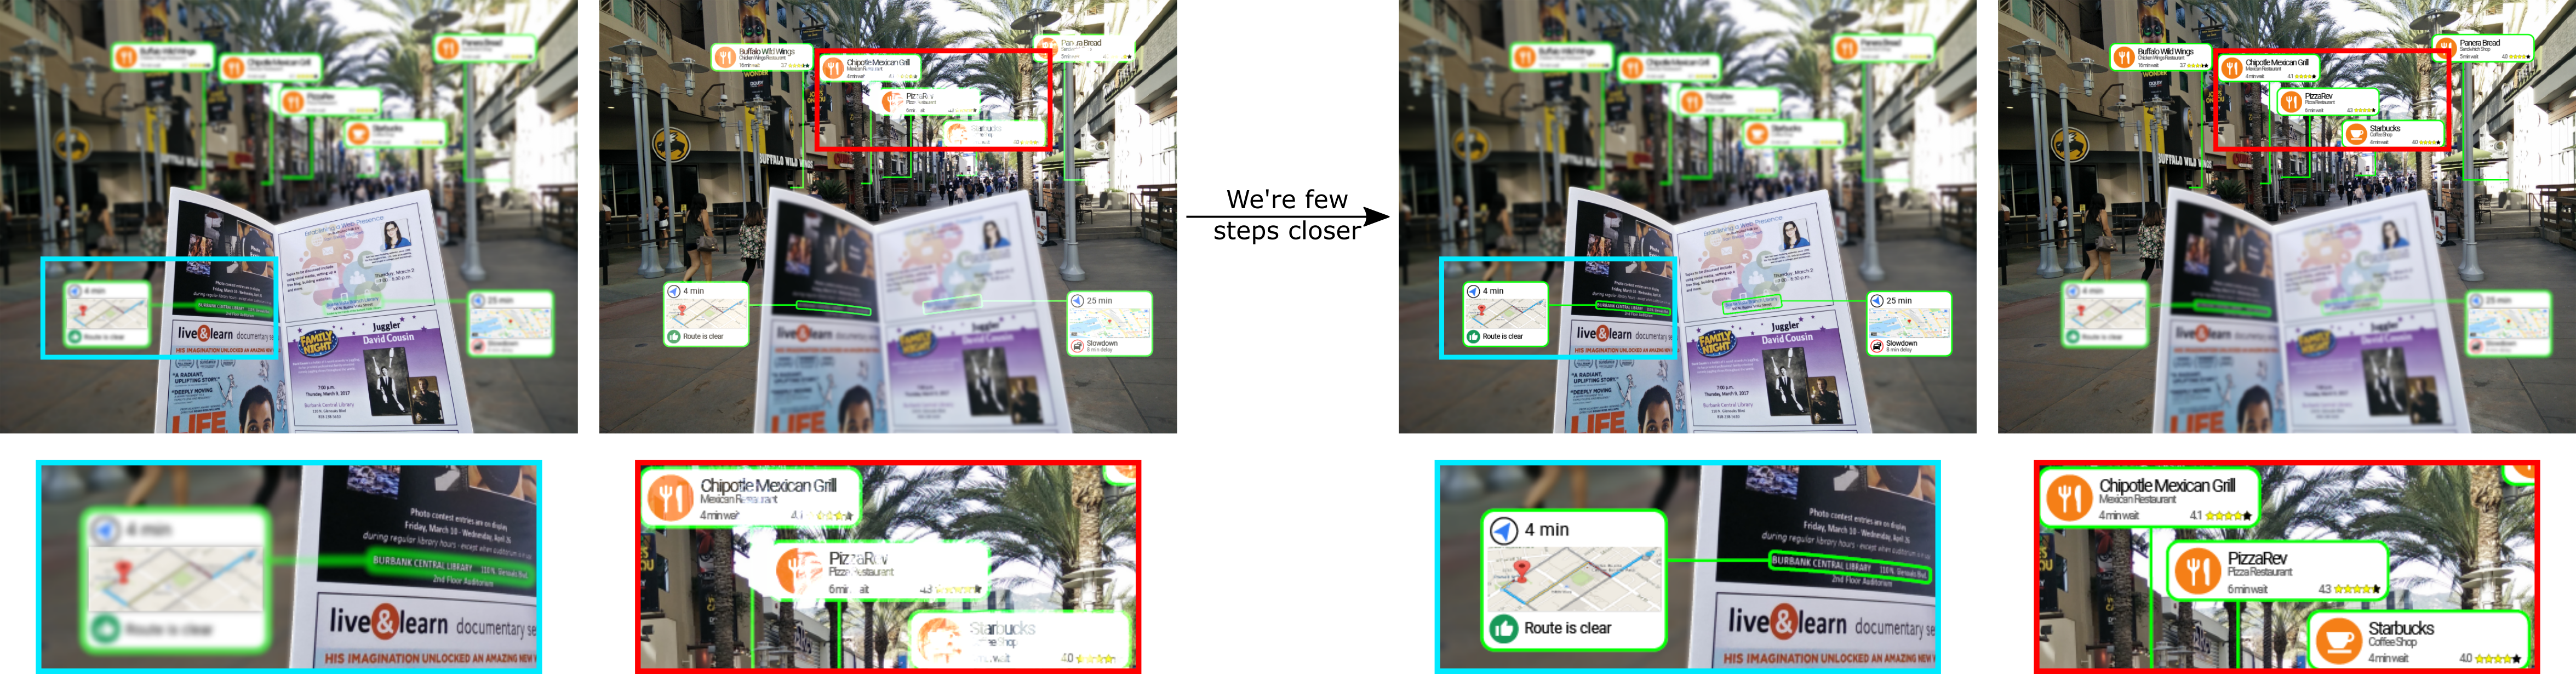
\includegraphics[width=0.99\columnwidth]{images/other/contributions}
\caption[Contributions of this dissertation]{Figures shows the contributions of this dissertation with a concept diagram. We've take small steps to go from the current state-of-the-art (on the left) to the envisioned future for augmented reality displays (on the right). Insests at the bottom row show enlarged portions of the regions of interest in the concept image above them. Image credit: Adapted from David Dunn.}
\label{fig:contributions}
\end{figure}


Fig.~\ref{fig:contributions} shows a concept augmented reality scene. In this concept scene, the real scene is composed of a pamphlet in the foreground and shops and restaurants in the background. To this scene, the current generation augmented reality displays can superimpose a transparent image at a fixed distance. However, the ultimate display as envisioned for augmented reality will be able to display multiple images at their correct depths with perceptually consistent depths. This dissertation takes a few steps towards realizing this vision.

\myblockquote{
The screen is a window through which one sees a virtual world. The challenge is to make that world look real, act real, sound real, feel real.
}{\cite{sutherland1965ultimate}}

Although the above quote is intended for Virtual Reality and considers multiple modalities (sight, hearing, haptics), it helps to convey the vision for Augmented Reality that I subscribe to. 
The ultimate Augmented Reality display would combine the real and the virtual worlds in a visually convincing manner—with consistent depth cues, latency, resolution, color fidelity, lighting, shadows, reflections, etc. 
Towards realizing this vision, this dissertation develops methods to improve monocular depth cues for Augmented Reality displays. 



% Bibliography
\input{common/references}

\appendix
\chapter[]{}
\section[]{Registration errors due to latency}
\label{sec:appendix:registration_errors_latency}

Suppose $\omega_{\text{head}}$ denotes the head rotation speed in degrees-per-seconds and $t_{\text{latency}}$ denotes the latency of the display system (i.e., the time between the tracking information used for rendering and the display of the currently rendered image), then the error of the currently displayed frame is:
\begin{equation}
    \theta_{\text{error}} = \omega_{\text{head}} \ast t_{\text{latency}}.
\end{equation}

For a virtual object that is displayed at distance $d_{\text{object}}$ away, the lateral error is given by:
\begin{equation}
    d_{\text{error}} = \tan(\theta_{\text{error}}) \ast d_{\text{object}}.
\end{equation}

Suppose $\omega_{\text{head}} = 150$ degrees-per-second and $t_{\text{latency}} = 10$ milliseconds, then $\theta_{\text{error}}=1.5$ degrees, and if $d_{\text{object}}=2$ meters, then $d_{\text{error}}=5.24$ centimeters.

\end{document}
